 \documentclass[a4paper]{article}
\usepackage[hmargin=1in, vmargin=1in]{geometry}
\usepackage{makeidx}
\usepackage{fancyhdr}
\pagestyle{fancy}
\usepackage[pdftex]{graphicx}
\usepackage{amsmath}
\usepackage{amssymb}
\usepackage{listings}
\usepackage{natbib}
%\usepackage{etex}
%\usepackage{m-pictex}
\makeindex
\begin{document}
\begin{center}
\title{Three dimensional coordinates into two dimensional coordinates transformation}\\
\author{Edward Gerhold}
Three dimensional coordinates into two dimensional coordinates transformation.
\date{\today}
\maketitle

Version 0.3.99 (From 2015, just removed the term functional, which was used in a wrong manner for a vector valued function)


\textbf{Remark. This is a development version. With proper mistakes.}

\end{center} 

\tableofcontents\\

\section{Introduction}

On a piece of paper you see three coordinate axes pointing into three
dimensions in space. In reality these vectors are two dimensional. Because
they point into \emph{three directions} on the 2-D paper,
and not into the real 3-D space. We take the sum of these three vectors 
times the coordinates as one new point.\\

\begin{figure}[ht]
\label{ijksystem}
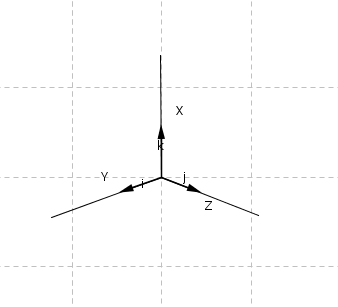
\includegraphics[scale=2]{figures/ijksystem.png}\\
\caption{Picture of a right handed 3-D coordinate system with ijk-basis-vectors on the axes pointing (imaginary)
into three dimensions. See \cite{Corral1} for introduction.}
\end{figure}

In this document we will design a ${2\times{3}}$ operator for linear map from the 3-D world onto a 2-D plane.
This linear map is designed after the pen-and-paper method to draw a 3-D coordinate system. I had the idea
to try out a 3-D coordinate system with three 2-D axes, because the axes on the paper are 2-D lines. And 
because the unit circle is available on the plane and because i have had learned some trigonometry recently, i 
had been able to arrange the axes around the origin onto a circle line.

It is assumed, that the input is from some set in $\mathbb{R}^{3}$. Say, some vertices of a 3-D object, or a set of points of a multivariate function plotting a 3-D surface. The result can be interpreted by the $\mathbb{R}^{2}$ standard basis. For example you can connect the 2-D points on the 2-D canvas with lineTo and fill the spaces beetween. 

\textbf{What we will do in the document}

\begin{enumerate}
\item We choose angles $\varphi$ for our coordinate axes. We can rotate our three axes freely around the unit circle.
\item We choose the unit length $r$ for the range unit on the axis. For all, two or each. This is like leaving normalized range.
\item We write down three vectors derived from the canonical basis vector $r(cos \theta, sin \theta)^{T}$, applying our angles and unit lengths.
\item We assemble a matrix $\boldsymbol{A}$ with the axis vectors. For a point by point transformation.
\item We read the example source code for a computer function, which is exactly two lines long. One line is for the new $x$-coordinate and one line of code is for the new $y$-coordinate.
\item We get the proofs for the linear behaviour of the transformation. And that 0 stays in 0. And a point on the axis on the axis.
\item We read other mathematical versions of the transformation. As a function, for example. And we will find connections between.
\item We derive the generic case of transforming coordinate systems down to the plane.
\item We will get some info about the background and environment of the transformation, which is explored by the author
\end{enumerate}\\

\textbf{Warning! Still foreign author.}\\
Edward Gerhold, who is writing this document, is nativly speaking german. His english, formerly very good, is not up to date yet.
And maybe this text contains phrases, he understands, at which no one in England, America or Australia, would be sure to understand.
%\chapter{1}

\section{Designing a $\mathbb{R}^{2\times{3}}$ coordinate system for our transformation from $\mathbb{R}^{3}$ to $\mathbb{R}^{2}$}

What can i say, what is $\mathbb{R}^{2\times 3}$? Is it the 2x3 matrix, or also a vector with three two dimensional vectors inside?
Can an element of $\mathbb{R}^{2\times 3}$ also be vector of vectors? Is 2x3 also a two dimensional plane with three coordinates? Yes, i think, it is so. 

The 2x3 matrix looks like the big body  around the three vectors had been transposed and they keep vertical orientation. Or is it the same, because it is the matrix itself, which is written like this. When i dot two vectors, they are both vertical. The same operation with a matrix is perpendicular, but absolutly equal in the writing and the result. Is $\mathbb{R}^{2\times 3}$ maybe the same in both cases? 

\subsection{The $_{n}$ indices $_x,_y,_z$ with $_x=1$, $_y=2$ and $_z=3$ for the components equal as for the vectors $\vec{e}_n$}
\index{index}

The index $_{n}$ in $r_{n}$, $\varphi_{n}$, $\vec{e}_{n}$ is the index for $_x$,$_y$,$_z$. For example $\varphi_{n}$  stands $\varphi_x, \varphi_y, \varphi_z$. $r_{n}$ stands for $r_x$, $r_y$ and $r_z$. $\vec{e}_{n}$ is for $\vec{e}_x$, $\vec{e}_y$, $\vec{e}_z$ It is possible, that in the formulas $x,y,z$ and $1,2,3$ may be used interchangeably. For example, when summing up the products of the coordinate components with the basis components, this happens. The formula is $\sum_{i=1}^{3}\vec{x}_{i}\vec{e}_{i}$, which is a sum of $x,y,z$ and the $\cos \varphi_{n}$ terms in the first components of $\vec{e}_{n}$ for $x$ and a sum of $x,y,z$ and the $\sin \varphi_{n}$ terms in the seconds components of $\vec{e}_{n}$ for $y$.\\

Being on point explaining indices, i should also explain this. The coordinates $x,y,z$ in the vector $\vec{x}$ are the same as the components $\vec{x}_{1},\vec{x}_{2},\vec{x}_{3}$. And the components $x, y$ in $\vec{y}$ are equal to $\vec{y}_{1}, \vec{y}_{2}$.\\

Throughout the text vector x is the input vector, vector y is the output vector. x,y,z and x,y use the same letters for points in space and in the plane.

\subsection{$\varphi_{n}$ the angles for the coordinate axes}

"Why do we need angles?" may be the first question. By rotating a vector around the origin, with the tip of the arrow on the circle line, and the tail in the origin, we can let the vector point into any chosen direction. Three of these vectors form the 3-D coordinate system. Each of the three vectors is an axis. The length of one unit on the axis is as long as the vector is, namely the
radius of the circle is the unit of the coordinate system axes.

\begin{figure}[ht]
\label{handsystems}

\includegraphics{figures/handsystems.png}
\caption{A right handed (z-up) and a left handed coordinate system. They just have different angles in our 2-D projection.}
\end{figure}

Whether the angles have to be measured in degrees or in radians, that depends on the cosine and sine functions you use.
And on how you would like to read your own definitions.\\

\fbox{We will arrange the three axes for x, y and z around the circle. By choosing an angle for each axis.}\\

Let $\varphi_{n}$ be the set of axis angles. There exists one angle for each axis. I put them into a set in this document to simplify the access. By using the subscript index $_{n}$ in numbers or letters, as $_x, _y, _z$ or $1,2,3$. $\varphi_x$ or $\varphi_1$ is the angle of the x-axis. $\varphi_y$ or $\varphi_2$ is the angle of the x-axis and $\varphi_z$ or $\varphi_3$ is the angle of the x-axis. \\

\begin{displaymath}
\begin{align}
\varphi_{n} :=& \{\varphi_x, \varphi_y, \varphi_z\ | \varphi_n \mbox{are angles for the three 2-D axis vectors}\}\\
 =& \{ \varphi_1, \varphi_2, \varphi_3 | \varphi_n \mbox{are angles for the three 2-D axis vectors} \}
\end{align}
\end{displaymath}

The angles are going around a circle. We can give any real number. The intervals are limited to a modulus operation internally. We can say, that $\varphi_n \in [0,2\pi)$ in radians. Or that $\varphi_n \in [0,360)$ in degrees. And that $\varphi_n \in \mathbb{R}$. We will need the three angles for the axes in short time. So don´t forget over the next lines.\\

\subsubsection{Degrees or radians?}

Maybe you have to convert the angles beetween degrees and radians. It depends on the cosine and sine functions, you use. For example, the JavaScript \emph{Math.cos($\varphi$)} and \emph{Math.sin($\varphi$)} functions take radians. Most other programming languages, too. For this reason i have written some examples.\\

\begin{example}
\textbf{Definition 1}
The function rad converts degrees to radians, it´s useful for computer functions taking radians.
\begin{displaymath}
\text{rad}(\phi) := \frac{\pi}{180} \times \phi, \phi \in \mathbb{R}
\end{displaymath}

\textbf{Example 2}
\label{120_degrees}

Here is an example of three angles. The three axes have an angle of 120 degrees between each neighbour axis. We start counting from the horizontal x-axis counterclockwise with positive numbers in radians, or negative numbers, if we go clockwise. We have to add each angle 120 degrees, after choosing our first angle.\\
 
\begin{displaymath}
\varphi_x = \text{rad(210)}, \varphi_y = \text{rad(330)}, \varphi_z = \text{rad(90)}
\end{displaymath}

\begin{displaymath}
\varphi_x &= \frac{\pi}{180} \times 210 &= \frac{7\pi}{6},  
\varphi_y &= \frac{\pi}{180} \times 330 &= \frac{11\pi}{6}, 
\varphi_z &= \frac{\pi}{180} \times 90 &= \frac{\pi}{2} 
\end{displaymath}
\end{example}

\textbf{Definition 3}
The function deg converts conversely from radians to degrees. You multiply your value with the reciprocal of PI/180, namely 180/PI and get the opposite result of the rad function. This proves, that $deg(rad(x))=x$ and $rad(deg(x))=x$.\\

\begin{displaymath}
\text{deg}(\phi) := \frac{180}{\pi} \times \phi, \phi \in \mathbb{R}
\end{displaymath}

\textbf{Example 4}
The first example, Example 1, was about an a little bit rotated righthand coordinate system. Here are some angles for a lefthand system, which includes the third axis with exactly 45 degrees beetween the perpendicular x and y axis.\\

\begin{displaymath}
\varphi_x &= \frac{\pi}{180} \times 0 &= 0,  
\varphi_y &= \frac{\pi}{180} \times 90 &= \frac{\pi}{2}, 
\varphi_z &= \frac{\pi}{180} \times 45 &= \frac{\pi}{4} 
\end{displaymath}

If you would like to get hands on angles, cosines, sines, or need a refresher, \cite{Corral2} is a good choice. And as well \cite{Corral1} and \cite{Strang2} teach unit circles, polar coordinates, sines, cosines and wonderful mathematics.\\

\begin{figure}
\begin{tabular}{-l-l-l-l-l-l-}
Angle &     sin &   cos & tan & csc & sec & cot\\
$0^{\circ}$  &    $0$&  $1$&  $0$&  undefined&  $1$&  undefined\\
$30^{\circ}$ & $\frac12$ & $\frac{\sqrt{3}}{2}$ & $\frac{1}{\sqrt{3}}$ & $2$ & $\frac{2}{\sqrt{3}}$ & $\sqrt{3}$
$45^{\circ}$ & $$& $$& $$& $$& $$& $$\\
$60^{\circ}$ & $$& $$& $$& $$& $$& $$\\
$90^{\circ}$ & $$& $$& $$& $$& $$& $$\\
$120^{\circ}$ & $$& $$& $$& $$& $$& $$\\
$135^{\circ}$ & $$& $$& $$& $$& $$& $$\\
$150^{\circ}$ & $$& $$& $$& $$& $$& $$\\
$180^{\circ}$ & $$& $$& $$& $$& $$& $$\\
$210^{\circ}$ & $$& $$& $$& $$& $$& $$\\
$225^{\circ}$ & $$& $$& $$& $$& $$& $$\\
$240^{\circ}$ & $$& $$& $$& $$& $$& $$\\
$270^{\circ}$ & $$& $$& $$& $$& $$& $$\\
$300^{\circ}$ & $$& $$& $$& $$& $$& $$\\
$315^{\circ}$ & $$& $$& $$& $$& $$& $$\\
$330^{\circ}$ & $$& $$& $$& $$& $$& $$\\
\end{tabular}

\caption{Overview over the trigonometric function values. This table is written down from \cite{Corral2}.}
\end{figure}

\subsection{$r_{n}$ is the length of the unit on each axis}

It was possible to choose another name for the unit length on the axis. But to stay closely related to the basic operations, 
which are used for creating and applying the coordinate system, namely the formulas for the $(x,y)$ coordinates in polar coordinates,
i stick with the variable name $r_{n}$.\\

$r_{n}$ describes the length of the unit of one axis. Like with polar coordinates, the length of the vector from the origin to the $(x,y)$ pair on the unit circle, gets increased to the length of $r_{n}$.

\begin{displaymath}
r_{n} := \{ r_{x}, r_{y}, r_{z} | r_n \mbox{ is the unit for $1$ on each axis }\} = \{ r_{1}, r_{2}, r_{3} | r_n \mbox { is the unit each axis } \}
\end{displaymath}

There is a bit to mention about the r-value:\\

\begin{enumerate}
\item The axes have $\|\vec{e}_{n}\|_{2}=1$ if you set $r_x = r_y = r_z = 1$. This gives mathematical unchanged results.
\item If you set $(r_x = r_y = r_z) > 1$ you scale the image by that factor, if it is $(r_x = r_y = r_z) < 1$ you shrink the graph.
	The mathematical results get changed.
\item If you set all r-values to different lengths, rotation of objects inside the coordinate system look unrealistic. For that use a 		local basis for each object and set the coordinate system itself again to r-values equal on all axes.
\item If you the the r-values to different lengths than $1$, all mathematical results get changed and the whole examination is more 	  complicated, and maybe not solvable, since we got it to do with an non-invertible operator.
\end{enumerate}

In short $\|\vec{e}_{n}\| = r_n$, and the best option is, to set all three axes to normalized length of $1$.\\

 The coordinates can be scaled independently from the transformation by multiplying the 2-D points with a zoom factor, which can be $z > 1$ to enlarge, or $\frac{1}{z}$ to scale down. This factor can be applied by the drawing function instead of by us.\\

\fbox{The number $r$ is for the length of one unit on each axis. $r_x=r_y=r_z=1$ is optimal.}\\

\fbox{If you want to measure data you should stick with unit length of 1.}

\subsection{$\vec{e}_{n}$ are the three 2-D axis vectors which are like basis vector}

We have drawn some axes on a piece of paper and taken the angles starting from zero counterclockwise on the x-axis.
We know now, that elonginating an axis vector by changing the radius forces us to draw one circle for each axis. You see the
unit ball with the diameter of $2$ and a radius of $1$ which is $r$. But visually it is not there, if you use the coordinate system.\\

Now we will write down the three basis vectors. Each vector points from the origin onto the circle line of its axis. With the same
values on alle axes, in the document we will use the unit length of $1$, they share the same circle on the first unit. And no matter how you rotate them, on all units. We will still map 3-D coordinates with three 2-D axes onto the 2-D screen.

Let $\vec{e}_{n}$ be the set of three two dimensional basis vectors. In this document and some literature and scripts,
we call them $\vec{e}_x$, $\vec{e}_y$ and $\vec{e}_z$. Another well known names for the basis vectors are $\vec{i}$, 
$\vec{j}$ or $\vec{k}$ for example. That is equal to the picture of the coordinate axes at \ref{ijksxstem} in this document.\\

Multiplying the 2x3 basis with the 3x1 points later results in wonderful 2x1 points. We will see it as a function, some flipping of the derivatives and the integral over the e-vector function doing the coordinate transformation after upgrading by adding the coordinate by the rules of integration.\\

\begin{displaymath}
\vec{e}_{n} := \{\vec{e}_x, \vec{e}_y, \vec{e}_z | \vec{e}_{n} \mbox{are the coordinate axes} \} = \{\vec{e}_1, \vec{e}_2, \vec{e}_3  | \vec{e}_{n} \mbox{are the coordinate axes} \}\\
\end{displaymath} 

This is now a set of the three axis vectors. We give them the letter $e$ and a subscript for the coordinate component in the numeric order of $x=1, y=2, z=3$. To arrange these vectors we already got around the unit circle and layed them out there. To measure the angles, beginning on the horizontal coordinate axis or zero, until we reach the vector. The vectors point into the positive direction of the described axis.\\

\begin{figure}[ht]
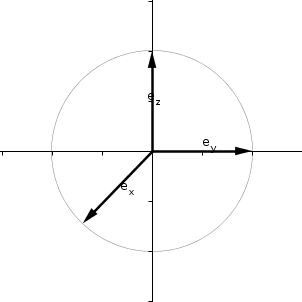
\includegraphics[scale=0.8]{figures/righthand45.png}
\caption{The three basis vectors point into the positive directions of the desired coordinate axes each. They are arranged around a circle with the trigonometric functions of cosine and sine. The coordinate system shown is a righthanded coordinate system.}
\end{figure}

\begin{figure}[ht]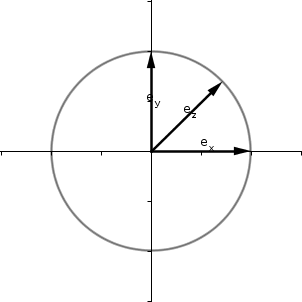
\includegraphics[scale=0.8]{figures/lefthand45.png}
\caption{The three two dimensional basis vectors as a lefthanded coordinate system.}
\end{figure}

To reach all three (x,y) at the tips of the vectors, we will now pull out the cosine and sine functions and stuff them together
with $r$ and $\varphi$ into a 2x1 vector with two components. So any (x,y) on one line from the origin to far distance can be reached like in polar coordinates\footnote{Interested readers may find in \cite{Corral1}, \cite{Corral2} and \cite{Strang2} everything about polar coordinates, parametrization of x and y with cosine and sine, the unit circle and the distance or radius r and more to these topics.} with the following parametrization.\\

\begin{displaymath}
\left(\begin{array}{1}x\\y\end{array}\right) = \left(\begin{array}{1}r \cos \varphi\\ r \sin \varphi\end{array}\right)\\
\end{displaymath}\\

Which can alternativly be written like $(x,y) = (r \cos \varphi, r \sin \varphi)$.\\

Modeling the three two dimensional basis vectors with this information,
we get the following three two dimensional basis vectors. They point along the coordinate axes and are the ruler for our transformation.\\

\begin{displaymath}
\vec{e}_x := (r_x\cos(\varphi_x), r_x\sin(\varphi_x) )^T = \left(\begin{array}{1}r_x\cos(\varphi_x)\\r_x\sin(\varphi_x) \end{array}\right)\\
\end{displaymath}
\begin{displaymath}
\vec{e}_y := (r_y\cos(\varphi_y), r_y\sin(\varphi_y) )^T = \left(\begin{array}{1}r_y\cos(\varphi_y)\\r_y\sin(\varphi_y) \end{array}\right)\\
\end{displaymath}
\begin{displaymath}
\vec{e}_z := (r_z\cos(\varphi_z), r_z\sin(\varphi_z) )^T = \left(\begin{array}{1}r_z\cos(\varphi_z)\\r_z\sin(\varphi_z) \end{array}\right)\\
\end{displaymath}\\

Each component of (x,y,z) has now it`s own basis vector. By multiplying the cos terms for the x and the sin terms for y with the corresponding component of (x,y,z) and summing the three products up for each of x and y, we directly obtain the right coordinate on the plane. All we would have to do is to connect the points again, or to fill the space between. \\

\begin{figure}[ht]
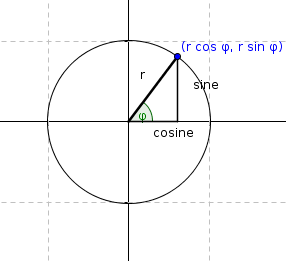
\includegraphics[scale=2]{figures/unitcircle.png}
\caption{A picture of the unit circle, the hypotenuse r, the adjacent cosine, the opposite sine and the angle $\varphi$. It is a circle of radius r, and no longer the unit circle, if $r \neq 1$.}
\end{figure}



\subsection{Now we need the vector basis theorem}\\

\subsubsection{The general formula for importing a vector into a coordinate system}

Last section i am talking about multiplying the coordinates with the new vector basis. Which i state to be the same as the coordinate system, we drew on a piece of paper at the beginning. We wrote down the angles, made out the unit length, and wrote down the three basis vectors with the information. Where is this coming from?\\

Every mathematics, physics or related course has a lesson, where the orthogonal basis of an object it's coordinate system is introduced. Orthogonality has some wonderful properties, and solving differential equations and other complicated systems take help from orthogonal vector sets.\\

A orthogonal basis is a set of 2 or three or up to infinite orthogonal (perpendicular) vectors. They describe the coordinate system, the space, the dimensions, and one has to show for excercises, that the basis is linearly independent, that each basis vector points into it´s own dimension and not into the others. \\

Another excercise is to orthogonalize the existing vectors with Gram-Schmidt. Interested readers will find it in \ref{gram_schmidt_excercise} \\

We want to design a coordinate system with three coordinates and two dimensions. At least one vector has to be linearly dependent of both basis vectors. We want to design a basis, or better a linear mapping, or best a coordinate system, which is a mix of both dimensions. We will use cosine and sine. We combine the three coordinates for three proportional horizontal moves. We combine the three coordinates for three vertical moves. Proportional to the coordinates and possibly with positive or negative amounts (up or down with sine, right or left with cosine) depending on the direction of the coordinate axis.\\

Remark. My article broke in when first time touching the linear dependence after being sure this formula works and "i have got some basis, right?". But i think, we are making progress. Now let us continue designing the axis vectors. We will look at the formula now.\\

The one lemma we need is this general theorem for multiplying a vector with the a basis of a target coordinate system.\\


\newtheorem{Vectorbasis}{Theorem. Hamel basis}
\begin{Vectorbasis}
A subset X of a linear vector space E is called a Hamel basis of E if every vector $x \in E$ can be uniquely expressed as a finite linear combination of some elements of X.
\begin{displaymath}
x=\sum_{k=1}^{n}a_{k}x_{k}
\end{displaymath}
for some nonzero scalar $a_{k}$ and vectors $x_{k} \in X$.
\end{Vectorbasis}
from \cite{Vershynin1}

The first time i had the idea, it was, "now try multiplying the coordinates with a basis." "But hey, they must be 2-D."\\

The plane gives us two possible directions, to go horizontal or vertical. And in a cartesian coordinate system with infinite points, we can choose any direction around a center point (x,y). Which is in the case of our coordinate system the origin at (0,0,0) or (0,0). We will see later, that the zero vector stays in the origin fo both systems.
Any not straight move will go horizontally or vertically by componentwise amounts. Any straight move horizontally or vertically will go by one of the components only.\\

\begin{figure}
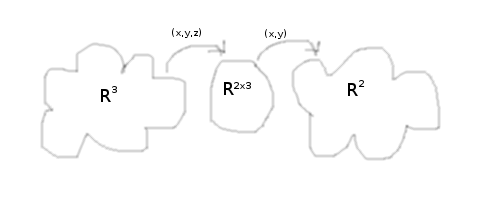
\includegraphics{figures/mediator.png}
\caption{A temporary picture of the process. We multiply the 3-D points with the 2x3 matrix and get the 2-D points back.}
\end{figure}

The point is, the general formula holds with a 2x3 basis.\\

\fbox{By taking 2-D vectors for three coordinates, we map directly onto the plane.}\\

\begin{figure}
\begin{displaymath}
    \boldsymbol{E}_{\mathbb{R}^2} = \begin{pmatrix}1 & 0 \\ 0 & 1\end{pmatrix}    \mbox{          }
    \boldsymbol{E}_{\mathbb{R}^3} = \begin{pmatrix}1 & 0 & 0\\ 0 & 1 & 0 \\ 0 & 0 & 1\end{pmatrix}    
    \boldsymbol{E}_{\mathbb{R}^{2\times3}} &= \begin{pmatrix}r_x\cos\varphi_x&r_y\cos\varphi_y&r_z\cos\varphi_z\\r_x\sin\varphi_x&r_y\sin\varphi_y&r_z\sin\varphi_z\end{pmatrix} \\
  \boldsymbol{E}_{\mathbb{R}^{2\times3}}_{225^{\circ}xrhs} = \begin{pmatrix}-\sqrt{\frac12}&1&0\\-\sqrt{\frac12}&0&1\end{pmatrix}     
\end{displaymath}
\caption{The standard basis for the $\mathbb{R}^{2}$ spans up the two dimensional space. When the three coordinates, which were a linear combination of $\lambda\begin{pmatrix}1\\0\\0\end{pmatrix} + \mu\begin{pmatrix}0\\1\\0\end{pmatrix} + \nu\begin{pmatrix}0\\0\\1\end{pmatrix}$ are combined into two coordinates, they become a linear combination of $\lambda\begin{pmatrix}1\\0\end{pmatrix}$ and $\mu\begin{pmatrix}0\\1\end{pmatrix}$. For sure, $\lambda$ is the sum of the cosine terms with the coordinates and $\mu$ is the sum of the sine terms with the coordinates in the two dimensions. }
\end{figure}

The formula for multiplying a vector with a basis to get a new vector is this.\footnote{The formula can be found in many mathematics, chemistry and physics lecture scripts, and a good introduction is \cite{Strang1}.}\\

\begin{displaymath}
\vec{y} = \displaystyle\sum_{i=1}^{n} \vec{x}_{i}\vec{e}_{i}
\end{displaymath}

This is the same formula for the linear combination in general.\\

It is done componentwise for each row of the vector. $n$ is the number of the source dimensions. In our case it is $n = 3$. 
We are summing three products for each component of the new vector. Our old $\vec{x}$ is a $\vec{x} \in \mathbb{R}^3$.\\
With $\vec{x}_{i}$ as the coordinate component and $\vec{e}_{i}$ as the corresponding basis vector in the right component. 
$\vec{y}$ is the resulting new vector.  The new vector $\vec{y}$ is a $\vec{y} \in \mathbb{R}^2$.\\

In our scenario is $V \subset \mathbb{R}^{3}, \vec{x} \in V$ and $W \subset \mathbb{R}^{2}, \vec{y} \in W$.\\

\subsubsection{Connection to ijk-Notation}

This is also equal to\\

\begin{displaymath}
\vec{x} = x\vec{i} + y\vec{j} + z\vec{k}
\end{displaymath}

what also explains, what the ijk-Notation means. If you don´t use it already for determining determinants for
calculating cross products (\ref{crossproducts}). It is for describing a vector. Don´t forget, our $i, j, k$ basis is two dimensional, 
because we draw on a 2-D plane like the computer screen or a piece of paper. \\

With a 3x3 basis the vector $x\vec{i} + y\vec{j} + z\vec{k}$ is equal to \left(\begin{array}{1}x\\y\\z'\end{array}\right)$. But with a 2x3 basis the vector $x\vec{i} + y\vec{j} + z\vec{k}$ is becoming  \left(\begin{array}{1}x\\y\end{array}\right)$\\

\subsubsection{Coordinate system}

\subsection{Time to show the operation}

The operation of multiplying the (x,y,z) coordinate with our $\mathbb{R}^{2\times{3}}$ coordinate axis vectors in order is the following:\\

\begin{displaymath}
\left(\begin{array}{1}x\\y\end{array}\right) = \left(\begin{array}{1}
xr_x\cos\varphi_x + yr_y\cos\varphi_y + zr_z\cos\varphi_z\\
xr_x\sin\varphi_x + yr_y\sin\varphi_y + zr_z\sin\varphi_z\end{array}\right)\\
\end{displaymath}\\

Right, this small formula brings over the $\mathbb{R}^{2\times{3}}$ the unexpected images of the preimage from $R^3$ to $R^2$.

Remark. Meanwhile i am ready to say $\mathbb{R}^{2\times{3}}$ image, and to believe, that this coordinate system is spanning the $\mathbb{R}^{2\times{3}}$ up (spread into the three dimensions) on the plane.\\

\begin{figure}[ht]
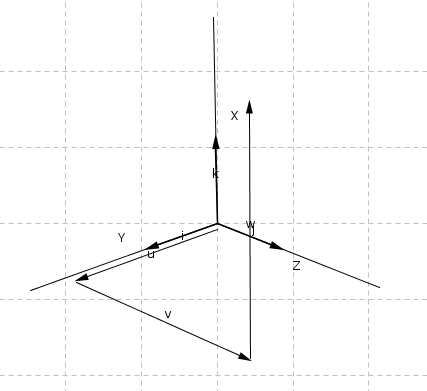
\includegraphics{figures/pathcoords.png}
\caption{The path a point goes from the origin. Along the first axis, then from that parallel to the second along that axis, and last parallel to the third axis as many units as the coordinate says. You can not see on this picture, how it is deconstructed by cosine and sine into left and right moves. To see, just draw the two missing sides of the triangles under each move. The z axis has a cosine of 0. I will paint a new picture for.}
\end{figure}\\

It is almost time to finish the matrix. And to go through a set of points. To draw the new set of resulting points.
For this i close the explaining chapters. And come to the part of the formal mathematical definitions. (Were i will
find alternatives for the matrix and related rules and laws, helpful for the understanding of the happenings.)\\

\textbf{Remark about the document structure.} \LaTeX and i are new to each other. For the theorems, proofs, defintions, corollaries, examples there is the possibility of a personal layout, which i have not prepared yet. And additionally, the following will contain some things, where real
mathematicians would start to smile. But i will do my best to correct any of my passages over the next time until i reach v1.0.0.\\

\section{The transformation $\mathbb{R}^{3} \rightarrow \mathbb{R}^{2}$ yields a perfect image}

\begin{figure}[ht]
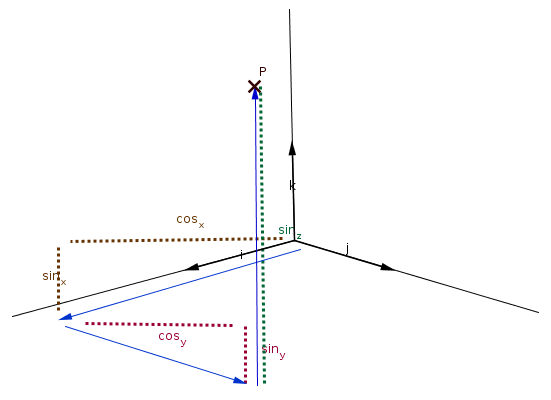
\includegraphics{figures/pathhacked.png}
\caption{The path a point goes from the origin. It is three moves horizontally and three vertically. One for each coordinate. Doing by scalar multiplication with the 2-D basis vector, all six proportional moves will be calculated, three of them build a weighted sum of a linear combination for interpretation of the $\mathbb{R}^{2}$ basis.}
\end{figure}\\

\subsection{Defining the Topology on the }

Remark. This subsection is started on July 31. And has still to be continued on Aug 20. Meanwhile i read a little of Munkres already and am fine, thanks.\\

Let $V$ be an open set in $\mathbb{R}^{3}$.\\

Let $B(\vec{x}, \epsilon)_{3}$ be a standard environment in the 3-space.\\

Let $W$ be an open set in $\mathbb{R}^{2}$.\\

Let $B(\vec{x}, \epsilon)_{2}$ be a standard environment in the 2-space.\\

Let the euclidean norm $\|\cdot\|_{2}$ be the default norm for three and two dimensions.\\

Let the $d(x,y)_{2} = \|x-y\|$ be the according metric.\\

Let $f:V\rightarrow W$ be a continuous function, and $A:V\rightarrow W$, $A \in L(V,W), Hom(V,W)$ be a rectangular matrix. Both map with equal operations V to W.\\

Let $V$ be the set of all points $(x,y,z) \in V \subset R^3$ which are about to become transformed. $V := \{ \vec{x}=(x,y,z)^T | x,y,z \in \mathbb{R}, \vec{x} \in V \subset \mathbb{R}^{3} \}$.\\

Let $W$ be the set of all points $(x,y) \in W \subset R^2$ which are the result of the transformation $W ;= \{ \vec{y}=(x,y)^T | \vec{y} \in W \subset \mathbb{R}^{2} x,y \in \mathbb{R}, \boldsymbol{A}\vec{x}=(x,y)^{T}\}$.\\

Remark. The topology has still to be defined extensivly in this document.\\

\subsection{Matrix version}

A $m\times n$ matrix is a rectangle or square of numbers.\\
\begin{displaymath}
    \boldsymbol{A} = (a_{ij})_{i,j \in \mathbb{N}^{+}} = \begin{pmatrix}a_{11} & ... & a_{1n}\\\vdots&\ddots&\vdots\\a_{m1} & ... & a_{mn}\end{pmatrix}
\end{displaymath}\\

Matrix with vector multiplication, from left to right in the matrix and from top to bottom in the vector, and that row by row, is achived by \\

\begin{displaymath}
    \boldsymbol{A}\vec{x} = (\sum_{j=1}^{n}a_{ij}\vec{x}_{j})_{i = 1..m} = \begin{pmatrix}a_{11}v_{1} + a_{12}v_{2} + ... + a_{1n}v_n\\\vdots \\a_{m1}v_{1} + a_{m2}v_{2} + ... + a_{mn}v_n\end{pmatrix} = \left(\begin{array}{1}w_{1}\\\vdots\\w_{m}\end{array}\right) = \vec{y}

\end{displaymath}\\

This formula is not much different from the multiplication with a vector basis, but it also accounts for the rows in the formula. The vector basis multiplication implies the componentwise row operations by using vectors.\\

\index{Definition}
\newtheorem{Definition}{Definition}
\begin{Definition}

Let \boldsymbol{A} be the matrix containing the three, two dimensional and trigonometric, basis vectors in order, one each
column. You get a rectangular 2x3 matrix $\boldsymbol{A} \in \mathbb{R}^{2\times{3}}: \mathbb{R}^{3} \rightarrow \mathbb{R}^{2}$. With the coordinate axis vectors $\left(\begin{array}{1}r_{n} \cos \varphi_{n}\\r_{n} \sin \varphi_{n}\end{array}\right)$ in the three columns. \\

\begin{displaymath}
\boldsymbol{A} := \begin{pmatrix}
    \vec{e}_x & \vec{e}_y & \vec{e}_z
    \end{pmatrix}
    = 
    \begin{pmatrix}
    r_x\cos(\varphi_x) & r_y\cos(\varphi_y) & r_z\cos(\varphi_z) \\
    r_x\sin(\varphi_x) & r_y\sin(\varphi_y) & r_z\sin(\varphi_z) \\
    \end{pmatrix}
\end{displaymath}\\
\end{Definition}


Remark. If $r_x = r_y = r_z$ you can pull out $r$ and write it in front of the matrix or multiply after transformation. A possible redefinition of the r-value is approaching. Remark of August 8.

%Remark. The operator definition should be defined differently.\\

%\newtheorem{DefinitionOperator}{Definition. A is a linear operator}
%\begin{DefinitionOperator}
%$\boldsymbol{A}$ is the linear operator $\boldsymbol{A} \in \mathbb{R}^{2\times{3}} : \mathbb{R}^3 \rightarrow \mathbb{R}^2$. This %operator maps coordinates from a subset of the $\mathbb{R}^{3}$ to the $\mathbb{R}^{2}$. ($\vec{x}) \mapsto \boldsymbol{A}\vec{x}$. 
%This operator is a matrix. But this operator is not invertible, because it is not square. It is not needed to be square, because we %map directly from the preimage to the image. The operator is mapping surjective, but since we interpret three dimensions on two, %there may be covered points on the plane, or overlaying of whole planes.
%\end{DefinitionOperator}\\

Remark. I commented the "linear map operator" definition out (linear map and operator is correct), because i have to write it again.


%Remark. About the matrix norm $\|A\|_{Frob}$. The number, after counting the components squares together and pulling the root is %$\sqrt{3}$. Pulling the norm chapter out of the introduction and introducing the measurements and estimations, also to myself, is %new on the TODO.


\index{Theorem}
\newtheorem{Theorem}{Proposition. My fundamental theorem of transforming 3-D Points into 2-D Points (Matrix)}
\begin{Theorem}
\label{Theorem}
If you multiply \boldsymbol{A}, the 2x3 matrix of the three two-dimensional basis vectors,
with the three-coordinate point $(x,y,z)$, the result is a two coordinate point, 
$(x,y)$. This point $(x,y)$ is the correct point on the two dimensional plane,
representing the point $(x,y,z)$ from the three dimensional coordinate system, you are transforming.\\
\begin{displaymath}
\boldsymbol{A}\left(\begin{array}{1}x\\y\\z\end{array}\right) = \left(\begin{array}{1}x\\y\end{array}\right)
\end{displaymath}

Applying the operator \boldsymbol{A} transforms the point $(x,y,z) \in V \subset \mathbb{R}^3$ into a new point $(x,y) \in W \subset \mathbb{R}^2$. 

\textbf{Proof}:\\

\begin{displaymath}
\boldsymbol{A}\left(\begin{array}{1}x\\y\\z\end{array}\right) = (\sum_{j=1}^{3}a_{ij}\vec{x}_{j})_{i=1,2}
%\end{displaymath}
%\beg{in{displaymath}
&= \left(\begin{array}{1}xr_x\cos(\varphi_x) + yr_y\cos(\varphi_y) + zr_z\cos(\varphi_z)\\
xr_x\sin(\varphi_x) + yr_y\sin(\varphi_y) + zr_z\sin(\varphi_z)\\
\end{array}\right) = \left(\begin{array}{1}x\\y\end{array}\right)
\end{displaymath}

\begin{figure}[ht]
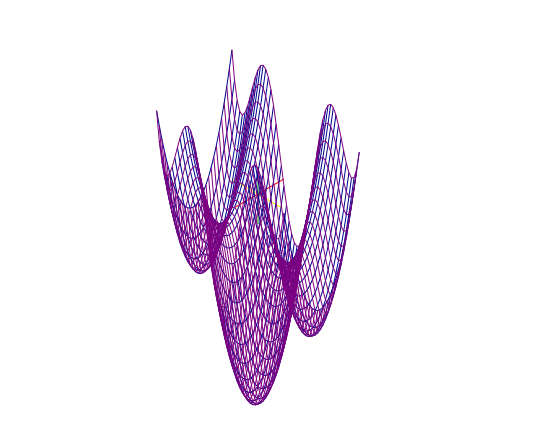
\includegraphics[scale=0.5]{figures/fxyplot.png}
\caption{$f(x,y) = x^2 + y^2 + 3y \sin y$ from [-5,5] and [-3,3] on a Canvas2DRenderingContext}
\end{figure}
\end{Theorem}


\subsection{Vectorbasis version}
\subsubsection{Hamelbasis with broken law of linear independence (or just a linear mapping)}

The theorem from Hamel says, that every vector space has a basis. And he gives a formula for this. The new vector in the new coordinate system is the sum of the coordinates multiplied with the basis vectors. \\

A Hamelbasis requires a linearly independent set of basis vectors. Which we can not provide. We change the dimension. The mapping yields the right image. So i will say, it is o.k. to break the rule of linear independence. This coordinate system is a special case.\\

\newtheorem{VectorBasisVersion}{Proposition. My fundamental theorem of transforming 3-D points into 2-D points (Vectorbasis)}
\begin{VectorBasisVersion}
If you multiply the three linear dependent two dimensional vectors with the three dimensional coordinates, they are mapped correctly onto the two dimensional coordinate system.
\end{VectorBasisVersion}

The operation is equal, but instead of working with three components in the new vector, we work with two components in the new vector. For each component, we build a sum of products. A sum of the productts of the basis components multiplied with the related coordinates ($x\vec{e}_x + y\vec{e}_y + z\vec{e}_z$), like we would do in the original form of this calculation with a $n\times n$ basis. \\

\begin{displaymath}
\vec{x} = \begin{pmatrix}x\\y\\z\end{pmatrix}
\end{displaymath}
\begin{displaymath}    
\vec{y} = x\vec{e}_{x} + y\vec{e}_{y} + z\vec{e}_{z}
\end{displaymath}    
\begin{displaymath}
    \sum_{i=1}^{n}\vec{x}_{i}\vec{e}_{i} = \left(\begin{array}{1}xr_x\cos(\varphi_x) + yr_y\cos(\varphi_y) + zr_z\cos(\varphi_z)\\
xr_x\sin(\varphi_x) + yr_y\sin(\varphi_y) + zr_z\sin(\varphi_z)\\
\end{array}\right) = \begin{pmatrix}x\\y\end{pmatrix} = \vec{y}
\end{displaymath}

The difference is that we have a dimension less than coordinates, and with that at least one axis, that must be a mix of the other two. By default our image in our coordinate system is a linear combination of $\lambda\begin{pmatrix}1\\0\end{pmatrix} + \mu\begin{pmatrix}0\\1\end{pmatrix}$, but before that, we map with a linear function from three dimensions to two dimensions, by using our coordinate system as or like a basis. \\

\newtheorem{VectorBasisBrokenLaw}{Proposition. Breaking the rule of linear independence to map from 3-D to 2-D}
\begin{VectorBasisBrokenLaw}
\label{broken_law_basis}
To transfer the points from 3-D to 2-D with the same formula, as mapping ordinary points with a vector basis into 
the corresponding coordinate system, it is o.k., to remove the third dimension from the basis and to multiply the
3-D coordinates with three 2-D vectors to get a correct mapping onto the projection plane.
\end{VectorBasisBrokenLaw}

\subsubsection{ijk-Notation Version}

The ijk-Notation is well known from describing vectors, from calculating cross products over determinants, from coordinate systems showing the normalized ijk vectors along the axes. The formula is this\\

\begin{center}
 $\vec{y} = x\vec{e}_{x}+y\vec{e}_{y}+z\vec{e}_{z}$
\end{center}

This is a very natural way. This is a real sum. The coordinates x,y,z multiply each a basis vector. This is the ordinary constant or scalar multiplication. Then the three scaled vectors are summed up together. This gives us a new vector, the sum of the three vectors. I have explained this already earlier, you can use this notation for this purpose, now it is time to repeat it. For a picture, look at figures \ref{ijksystem} and \ref{handsystems}.\\

\newtheorem{ijkVersion}{Proposition. The fundamental theorem of transforming 3-D points into 2-D points (ijk-Notation)}
\begin{ijkVersion}
If you write the vector down in ijk-Notation using the three two dimensional axis vectors, instead of three three dimensional linear independent basis vectors, the sum of the products with ijk and the coordinates, which is a new vector, equals the right vector on the 2-D plane.
\end{ijkVersion}

\textbf{Proof:}\\
\begin{displaymath}
 x\vec{e}_{x}+y\vec{e}_{y}+z\vec{e}_{z} = x\begin{pmatrix}r_x\cos\varphi_x\\r_x\sin\varphi_x\end{pmatrix} + y\begin{pmatrix}r_y\cos\varphi_y\\r_y\sin\varphi_y\end{pmatrix} + z\begin{pmatrix}r_z\cos\varphi_z\\r_z\sin\varphi_z\end{pmatrix} = \sum_{i=1}^{3}\vec{e}_{i}\vec{x}_{i} = \vec{y} = \begin{pmatrix}x\\y\end{pmatrix}
\end{displaymath}

\subsection{Function version}

The first days, i could not see the forest, because of all these trees. 
The operation can be written as function, or as part of a composition of functions.
The big thing for this point by point transformation is the easy usability. For example, 
to create surface plots and other function graphs from three dimensional space on a flat screen or printed paper.\\

\subsubsection{The linear vector valued $f(\vec{x})$}

We begin with $\vec{f}(\vec{x}) : V \subset \mathbb{R}^{3} \rightarrow \subset \mathbb{R}^{2}$. $\vec{f} \in V^{*}$\\


$f(\vec{x})$ is mapping the three dimensional coordinates onto our designed coordinate system. The multiplication of the components with the horizontal and vertical displacements which are represented by the axes of our coordinate system is the fix content of our function. Assume we have the angles and units designed and the function is well defined for its purpose.\\

\begin{displaymath}
\label{f_function}
\begin{align}
\vec{f}(\vec{x}) :&= \left(\begin{array}{1}\vec{x}_{1}r_x\cos\varphi_x + \vec{x}_{2}r_y\cos\varphi_y + \vec{x}_{3}r_z\cos\varphi_z\\					\vec{x}_{1}r_x\sin\varphi_x + \vec{x}_{2}r_y\sin\varphi_y + \vec{x}_{3}r_z\sin\varphi_z\end{array}\right)\\			
\end{align}
\end{displaymath}

This can even be written more convenient. The interested reader might find \cite{Corral1} and \cite{Strang2} useful. \\

\begin{displaymath}
\begin{align}
			\vec{f}(\vec{x}) = \vec{x}_{1}\begin{pmatrix}r_x\cos\varphi_x\\r_x\sin\varphi_x\end{pmatrix} + \vec{x}_{2}\begin{pmatrix}r_y\cos\varphi_y\\r_y\sin\varphi_y\end{pmatrix} + \vec{x}_{3}\begin{pmatrix}r_z\cos\varphi_x\\r_z\sin\varphi_z\end{pmatrix}
	\end{align}
\end{displaymath}


\newtheorem{FunctionVersion}{Proposition. My fundamental theorem of transforming 3-D points into 2-D points (Function))}
\begin{FunctionVersion}
The linear function (map) $\vec{f}(\vec{x})$ maps the points correctly from 3-D to 2-D. It is continuous in every point, the zero vector maps onto the zero vector. Passing a vector with three coordinates to the function results in a vector with two coordinates, which are the right coordinates on the 2-D screen.
\end{FunctionVersion}


\subsubsection{Composition of the functions $f \circ g$}

There are various possibilities to combine the output of g and the input of f.
The following functions are compositions of two functions and take some input and return our 2-D points.
f is transformingthe vector returned by g. g is taking the input in all examples and f is reworking the coordinates.
In other words, f is the same function as previously shown in \ref{f_function}.\\

\textbf{Example 1}\\

A call to $g(t)$ is returning a vector $\vec{x}$ passed to $f(\vec{x})$ by using the composition $f \circ g$ :  $f(g(t)) = \vec{y}$\\

\begin{displaymath}
\label{g_of_t_code}
g(t) := \left(\begin{array}{1}t\cos t\\t\sin t\\t\end{array}\right)
\end{displaymath}
Becomes the following
\begin{displaymath}
\begin{align}
			(\vec{f}\circ g)(t) := \cos t\begin{pmatrix}r_x\cos\varphi_x\\r_x\sin\varphi_x\end{pmatrix} + t \sin t\begin{pmatrix}r_y\cos\varphi_y\\r_y\sin\varphi_y\end{pmatrix} + t\begin{pmatrix}r_z\cos\varphi_x\\r_z\sin\varphi_z\end{pmatrix}
	\end{align}
\end{displaymath}

This is a 2-D image of a conical helix. You can look at Figure 14 how this looks like from $0$ to a few rounds of $2\pi$.\\

\begin{figure}
\label{g_of_t_figure}
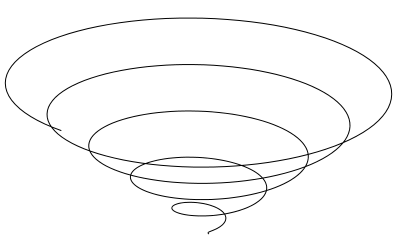
\includegraphics[scale=0.5]{figures/conicalhelix2.png}
\caption{This is $g(t)$ from \ref{g_of_t_code} in implement.html where implement.js from the repository is used once.}
\end{figure}

\textbf{Example 2}\\

 $g(x,y)=(x,y,z)$ this function will give us a surface plot. See figure \ref{g_of_x_y_figure}.\\

\begin{displaymath}
\label{g_of_x_y_code}
g(x,y) := \left(\begin{array}{1}x\\y\\e^{-x^{2} - y^{2}}\end{array}\right)
\end{displaymath}

That will be brought by $\vec{f}(\vec{x})$ into the following context. A function $(\vec{f}\circ g)(x,y) : E\times E \rightarrow W$.\\

\begin{displaymath}
\begin{align}
			(\vec{f}\circ g)(x,y) := x\begin{pmatrix}r_x\cos\varphi_x\\r_x\sin\varphi_x\end{pmatrix} + y\begin{pmatrix}r_y\cos\varphi_y\\r_y\sin\varphi_y\end{pmatrix} + e^{-x^{2}-y^{2}}\begin{pmatrix}r_z\cos\varphi_x\\r_z\sin\varphi_z\end{pmatrix}
	\end{align}
\end{displaymath}


\begin{figure}
\label{g_of_x_y_figure}
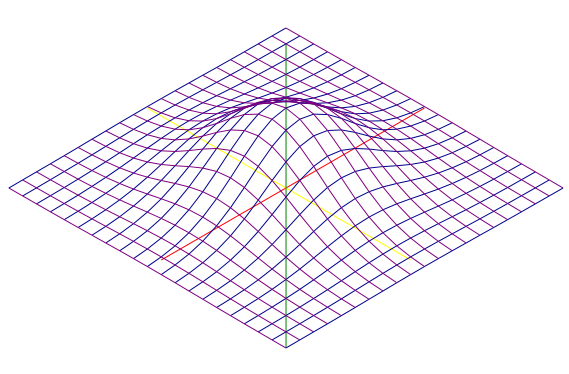
\includegraphics[scale=0.5]{figures/expfunction.png}
\caption{This is $\exp -x^{2}-y{2}$ from \ref{g_of_x_y_code} plotted with the cheap3danimate.html code within $[-2,2] \times [-2,2]$.}
\end{figure}

\textbf{Example 3}\\

A $g(x,y,z)$ or $g(\vec{x})$ a three-d or vector-valued function returning a three-d vector.\\

\begin{displaymath}
\label{g_of_x_y_z_code}
g(x,y,z) := \left(\begin{array}{1}x+1\\y\\z-1\end{array}\right)
\end{displaymath}

Which will become this kind of function. $(\vec{f}\circ g)(x,y,z) : E\times E \times E \rightarrow W$.\\

\begin{displaymath}
\begin{align}
			(\vec{f}\circ g)(x,y,z) := (x+1)\begin{pmatrix}r_x\cos\varphi_x\\r_x\sin\varphi_x\end{pmatrix} + (y)\begin{pmatrix}r_y\cos\varphi_y\\r_y\sin\varphi_y\end{pmatrix} + (z-1)\begin{pmatrix}r_z\cos\varphi_x\\r_z\sin\varphi_z\end{pmatrix}
	\end{align}
\end{displaymath}


The vector field of this formula is shown in figure \ref{vector_field_image}.

\begin{figure}
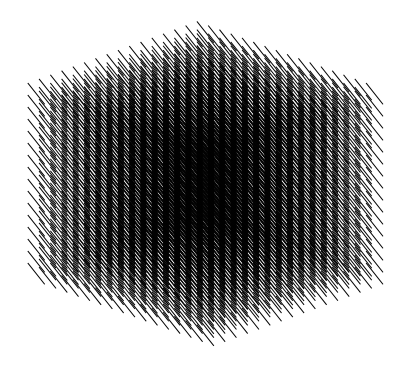
\includegraphics[scale=0.5]{figures/vectorfield.png}
\label{vector_field_image}
\caption{A 3-D vector field of a cubic section, this time of some random formula.}
\end{figure}

Remark. The vector field demo is primitive at this point.

\begin{center}
$g(\vec{x}) : \mathbb{R}^{3} \rightarrow \mathbb{R}^{3}$\\
$f(\vec{x}) : \mathbb{R}^{3} \rightarrow \mathbb{R}^{2}$\\
\end{center}


Remark. This section is not finished. Not only the plot for the vector field, some sophisticated demo with a physics formula, but the compositions are themselves not explained. Additionally in the section about differentiation, the compositions have to be veryfied.\\

\subsubsection{Vector valued function}
\label{vector_valued_func}

The book \cite{Corral1} defines a vector valued function like this:
\begin{displaymath}
f(t) = f_{1}(t)\vec{i}+f_{2}(t)\vec{j}+f_{3}(t)\vec{k}
\end{displaymath}

In our version this becomes a direct transformation onto the 2-D plane by using our 2x3 basis instead of a 3x3 basis.

\begin{displaymath}
f(t) = x(t)\begin{pmatrix}\cos\varphi_x\\\sin\varphi_x\end{pmatrix}
        +y(t)\begin{pmatrix}\cos\varphi_y\\\sin\varphi_y\end{pmatrix}
        +z(t)\begin{pmatrix}\cos\varphi_z\\\sin\varphi_z\end{pmatrix}
\end{displaymath}

Remak. The first chapter about differentiation, which follows later, deals with the constant form of $x(t), y(t), z(t)$. In a future version i will continue this topic with a few parametrized examples.\\

\subsection{Polar coordinate version}
\label{polar_coord_func}

The function can be written as a sum of three polar coordinate functions. The generic function for one component is this.

\begin{displaymath}
p(x, r, \theta) := xr\begin{pmatrix}\cos\theta\\\sin\theta\end{pmatrix}
\end{displaymath}

The sum of the three vectors gives us our correct position vector again.

\begin{displaymath}
P(x,y,z,r_x,r_y,r_z,\theta_x,\theta_y,\theta_z) :=  P(\vec{x}, \vec{r}, \vec{\theta}) := p(x, r_x, \theta_x)+p(y, r_y, \theta_y)+p(z, r_z, \theta_z)\\
\end{displaymath}

Well, i think this is ugly. And i should reconsider the r-value. Assuming the r-value be the usual normal unit length of 1, the functions become the following:

\begin{displaymath}
p_{n}(r, \theta) := r\begin{pmatrix}\cos\theta\\\sin\theta\end{pmatrix}
\end{displaymath}

And the whole combined function is again a sum of the three resulting 2-D vectors of the polar coordinate function.

\begin{displaymath}
P(\vec{x}) := p_{x}(x_{1}, \theta_{x}) + p_{y}(\vec{x}_{2}, \theta_{y}) + p_{z}(\vec{x}_{3}, \theta_{z})
\end{displaymath}



\subsection{Computer implementations of the transformation}
\subsubsection{Generic computer code (all you need)}

One of the \emph{main goals of this document} is to show the simplicity of transforming 3-D points into 2-D points for the use in small computer applications. For example for hand written small web applications. Say, you just want to draw a graph, 3-D on the 
2-D Canvas and do not have the need for WebGL, or it is not available on your old target systems, which was the reason for me, to try it myself anyways.\\

This should be in a border box.\\

\begin{example}
\fbox{
The following is example code for various computer systems.
}
\begin{lstlisting}
x_ = x*r*cos(alpha) + y*r*cos(beta) + z*r*cos(gamma)
y_ = x*r*sin(alpha) + y*r*sin(beta) + z*r*sin(gamma)
\end{lstlisting}\\
\fbox{ These are the one and only two lines of code you need.\\}

\end{example}\\

\newtheorem{CodeTheorem}{Only two lines of code needed to go from 3-D to 2-D points. (Computer Version)}
\begin{CodeTheorem}
The only two lines of code you need to convert the coordinates on the computer. The new x value
is summed up by multiplying each coordinate with the cosine term of the related axis vector. The new y value
is a sum of products of the coordinates with the sine terms of the related axis vectors.
\end{CodeTheorem}

\subsubsection{JavaScript computer code}
\begin{example}
This is a full EcmaScript 6 snippet with all neccessary informations.\\
\begin{lstlisting}
let rad = (deg) => Math.PI/180*deg;
let r_x = 1, r_y = 1, r_z = 1; 
let phi_x = rad(220), phi_y = rad(330), phi_z = rad(90); 
let xAxisCos = r_x*Math.cos(phi_x), 
    yAxisCos = r_y*Math.cos(phi_y),
    zAxisCos = r_z*Math.cos(phi_z),
    xAxisSin = r_x*Math.sin(phi_x), 
    yAxisSin = r_y*Math.sin(phi_y),
    zAxisSin = r_z*Math.sin(phi_z);
let transform2d = ([x,y,z]) => [
    x*xAxisCos+ y*yAxisCos+ z*zAxisCos,
    x*xAxisSin+ y*yAxisSin+ z*zAxisSin];
let transform2dAll = (P) => P.map(transform2d);

let examplePoints = transform2dAll([[1,2,3], [3,4,5], [14,24,15]]);
\end{lstlisting}
\end{example}\\
\fbox{ This is the realistic amount of code to write to transform all points from 3-D to 2-D.\\}

\begin{figure}[ht]
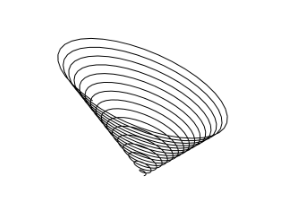
\includegraphics[scale=0.5]{figures/conicalhelix.png}
\caption{A conical helix (t/2*Math.cos(t), t*Math.sin(t), t) shown as (x,y,z)=f(t) with implement.html on a Canvas2DRenderingContext testing the javascript example code.}
\end{figure}

\section{Important proofs of the transformation behaviour}
\label{important_proofs}

A very important thing is to show, that the linearity of the transformation is in order. With a wrong function, bad thing can happen.
With the right functions, linear combinations should stay in the subspace.

\subsection{The origin stays in the origin}

A trivial proof is to prove, that the zero vector $\vec{0} \in \mathbb{R}^3$ maps to the zero vector $\vec{0} \in \mathbb{R}^2$.\\

\textbf{Proof}:
\begin{displaymath}
    \boldsymbol{A}\left(\begin{array}{1}0\\0\\0\end{array}\right)
    = \left(\begin{array}{1}0 + 0 + 0\\0 + 0 + 0\end{array}\right) 
    =\left(\begin{array}{1}0\\0\end{array}\right)
\end{displaymath}\\

\subsection{Points along one axis}

Another trivial proof is to prove, that coordinates lying on one axis are a multiple of the basis vector of the axis.\\

\textbf{Proof}:
\begin{displaymath}
    \boldsymbol{A}\left(\begin{array}{1}a\\0\\0\end{array}\right)
    = \left(\begin{array}{1}ar_x\cos \varphi_x + 0 + 0\\ar_x\sin \varphi_x  + 0 + 0\end{array}\right) 
    = a\vec{e}_x
\end{displaymath}

\begin{displaymath}
    \boldsymbol{A}\left(\begin{array}{1}0\\1\\0\end{array}\right)
    = \left(\begin{array}{1}0 + r_y\cos \varphi_y + 0\\0 + r_y\sin \varphi_y + 0\end{array}\right) 
    = \vec{e}_y
\end{displaymath}

\begin{displaymath}
    \boldsymbol{A}\left(\begin{array}{1}0\\0\\-b\end{array}\right)
    = \left(\begin{array}{1}0 + 0 - br_z\cos \varphi_z\\0 + 0 - br_z\sin \varphi_z\end{array}\right) 
    = -b\vec{e}_z
\end{displaymath}\\

\subsection{Multiplications with constants}

Another trivial proof is to show, that $\boldsymbol{A}(\lambda\vec{x}) = \lambda\boldsymbol{A}\vec{x}$. It doesn´t matter, where you multiply with the constant. You can multiply the original vector, or the resulting vector. You reach the same point.\\

\textbf{Proof}:\\
\begin{displaymath}
\begin{equation*}
\begin{align*}
\boldsymbol{A}(\lambda\vec{x}) &= \boldsymbol{A}\left(\begin{array}{1}\lambda{x}\\\lambda{y}\\\lambda{z}\end{array}\right)\\ &= \left(\begin{array}{1}\lambda{x}r_x\cos(\varphi_x) + \lambda{y}r_y\cos(\varphi_y) + \lambda{z}r_z\cos(\varphi_z)\\
\lambda{x}r_x\sin(\varphi_x) + \lambda{y}r_y\sin(\varphi_y) + \lambda{z}r_z\sin(\varphi_z)
\end{array}\right)\\
    &= \lambda\left(\begin{array}{1}xr_x\cos(\varphi_x) + yr_y\cos(\varphi_y) + zr_z\cos(\varphi_z)\\
xr_x\sin(\varphi_x) + yr_y\sin(\varphi_y) + zr_z\sin(\varphi_z)\\
\end{array}\right)\\
    &= \lambda\left(\begin{array}{1}x\\y\end{array}\right)\\
    &= \lambda\boldsymbol{A}\vec{x}
\end{align*}
\end{equation*}
\end{displaymath}\\


\subsection{Additions and subtractions}

Another trivial proof is to show, that $\boldsymbol{A}(\vec{x} + \vec{y}) = \boldsymbol{A}\vec{x} + \boldsymbol{A}\vec{y}$. 
It does not matter, if you add the original or the results . The outcome is the same point, the same vector.\\
 
\textbf{Proof}:\\

\begin{displaymath}
\begin{equation*}
\begin{align*}
\boldsymbol{A}\left(\begin{array}{1}x+u\\y+v\\z+w\end{array}\right) &= \left(\begin{array}{1}(x+u)r_x\cos(\varphi_x) + (y+v)r_y\cos(\varphi_y) + (z+w)r_z\cos(\varphi_z)\\
(x+u)r_x\sin(\varphi_x) + (y+v)r_y\sin(\varphi_y) + (z+w)r_z\sin(\varphi_z)\\
\end{array}\right)\\
            &= \left(\begin{array}{1}xr_x\cos(\varphi_x) + yr_y\cos(\varphi_y) + zr_z\cos(\varphi_z)\\
xr_x\sin(\varphi_x) + yr_y\sin(\varphi_y) + zr_z\sin(\varphi_z)\\
\end{array}\right) + \left(\begin{array}{1}ur_x\cos(\varphi_x) + vr_y\cos(\varphi_y) + wr_z\cos(\varphi_z)\\
ur_x\sin(\varphi_x) + vr_y\sin(\varphi_y) + wr_z\sin(\varphi_z)\\
\end{array}\right)\\    
    &= \left(\begin{array}{1}x\\y\end{array}\right) + \left(\begin{array}{1}u'\\v'\end{array}\right)\\
    &= \boldsymbol{A}\left(\begin{array}{1}x\\y\\z\end{array}\right) + \boldsymbol{A}\left(\begin{array}{1}u\\v\\w\end{array}\right)
\end{align*}
\end{equation*}
\end{displaymath}
\subsection{Rule of linearity}

\textbf{Corollary} From the previous two proofs, it is obvious to see, that
\begin{displaymath}
\boldsymbol{A}(\lambda\vec{x} + \kappa\vec{y}) = \lambda\boldsymbol{A}\vec{x} + \kappa\boldsymbol{A}\vec{y} = \lambda\left(\begin{array}{1}x\\y\end{array}\right) + \kappa\left(\begin{array}{1}u'\\v'\end{array}\right)\\
\end{displaymath}
which is a standard formulation of the rule of linearity. For example, you can find this rule in the form $\boldsymbol{A}(c\vec{x} + d\vec{y}) = c\boldsymbol{A}\vec{x} + d\boldsymbol{A}\vec{y}$ in \cite{Strang1}, but also in every linear algebra 1 lecture script.\\


\section{Corollaries}

\subsection{Converting four Dimensions down to two dimensions}\\

The proposed theorem can be used to handle more dimensions, for example can four two-dimensional
vectors represent a 4-D space on the 2-D plane. They get converted into the correct
2-D points by giving each dimension a direction vector around the unit circle and relying the
horizontal and vertical amounts of cosine and sine. For Example, if you use a 2x4 matrix 
and convert all points at each instance of $t$ you have a moving object into the direction 
of the fourth basis vector. \\

\begin{displaymath}
\boldsymbol{A} := \begin{pmatrix}
    \vec{e}_x & \vec{e}_y & \vec{e}_z & \vec{e}_t\end{pmatrix}\\ = 
    \begin{pmatrix}
    r_x\cos(\varphi_x) & r_y\cos(\varphi_y) & r_z\cos(\varphi_z) & r_t\cos(\varphi_t)\\
    r_x\sin(\varphi_x) & r_y\sin(\varphi_y) & r_z\sin(\varphi_z) & r_t\sin(\varphi_t)\\
    \end{pmatrix}
\end{displaymath}

Here the basis is four times of two dimensions. A 2x4 matrix with four two dimensional basis vectors, one for each axis.\\

\begin{displaymath}
\boldsymbol{A}\left(\begin{array}{1}x\\y\\z\\t\end{array}\right) = \sum_{n} \vec{e}_{n}\vec{x}_{n} = \left(\begin{array}{1}x\\y\end{array}\right)\\
\end{displaymath}

\textbf{Proof}:

\begin{displaymath}
\boldsymbol{A}\left(\begin{array}{1}x\\y\\z\\t\end{array}\right) &= \left(\begin{array}{1}
xr_x\cos(\varphi_x) + yr_y\cos(\varphi_y) + zr_z\cos(\varphi_z) + zr_t\cos(\varphi_t)\\
xr_x\sin(\varphi_x) + yr_y\sin(\varphi_y) + zr_z\sin(\varphi_z)+ zr_t\sin(\varphi_t)\end{array}\right)\\
\end{displaymath}
\begin{displaymath}
&= x\vec{e}_x + y\vec{e}_y + z\vec{e}_z + t\vec{e}_t &= \sum_{n} \vec{e}_{n}\vec{x}_{n} &= \left(\begin{array}{1}x\\y\end{array}\right)
\end{displaymath}\\

The same method can be used, to convert points or vectors from any other number of dimensions, down to the $xy$-plane. 
It can so be used in a general $m \times n$ case, where one goes from $n$ dimensions down to $m$ dimensions.\footnote{http://de.wikipedia.org/wiki/Abbildungsmatrix, shows the m by n case.} 

\subsection{Alternative definition of the transformation by using dot products}
\label{alternative_def_using_dot}
Underways, i came to another conclusion. If i pull the two row vectors out of the matrix and define them as two column vectors,
then i can dot each with the coordinate vector and write the dot product into the component of the resulting vector.\\

\begin{displaymath}
    \vec{x} = \left(\begin{array}{1}x\\y\\z\end{array}\right)       \vec{c} = \left(\begin{array}{1}r_x\cos\varphi_x\\r_y\cos\varphi_y\\r_z\cos\varphi_z\end{array}\right)            \vec{s} = \left(\begin{array}{1}r_x\sin\varphi_x\\r_y\sin\varphi_y\\r_z\sin\varphi_z\end{array}\right)
\end{displaymath}
 
\begin{displaymath}
    \vec{y} = \left(\begin{array}{1}\vec{x}\cdot\vec{c}\\\vec{x}\cdot\vec{s}\end{array}\right)
\end{displaymath}

The result is $\vec{y} \in W$, $W \subset R^2$.\\

This operation can also be extended into any finite number of dimensions, and will result in two coordinates then. Just add the dimensions to $\vec{x}, \vec{c}, \vec{s}$ and see.\\

\textbf{Proof}:

\begin{displaymath}
\left(\begin{array}{1}\vec{x}\cdot\vec{c}\\\vec{x}\cdot\vec{s}\end{array}\right) = \left(\begin{array}{1}
xr_x\cos(\varphi_x) + yr_y\cos(\varphi_y) + zr_z\cos(\varphi_z)\\
xr_x\sin(\varphi_x) + yr_y\sin(\varphi_y) + zr_z\sin(\varphi_z)\end{array}\right) = \left(\begin{array}{1}x\\y\end{array}\right)
\end{displaymath}


Meanwhile it is clear, that this operation is the same as $\nabla\vec{f}(\vec{x}) \cdot \vec{x}$, which is the natural dot product of the gradient vector of our linear function $\vec{f}(\vec{x})$ with the coordinate vector.

\section{Derivatives of $\vec{f}(\vec{x}) : V \rightarrow W$ }
\subsection{Derivative}

Again we begin with $\vec{f}(\vec{x}) : V \subset \mathbb{R}^{3} \rightarrow W \subset \mathbb{R}^{2}$.

\begin{displaymath}
\vec{f}(\vec{x}) := \left(\begin{array}{1}\vec{x}_{1}r_x\cos\varphi_x + \vec{x}_{2}r_y\cos\varphi_y + \vec{x}_{3}r_z\cos\varphi_z\\
\vec{x}_{1}r_x\sin\varphi_x + \vec{x}_{2}r_y\sin\varphi_y + \vec{x}_{3}r_z\sin\varphi_z\end{array}\right)
\end{displaymath}

The first derivatives after the vector are the following by using the product rule and partial differentiation. 
The scalar component of the input is gone, because the derivative is $1$ and the other summand of the derived product is zero, because the cosine or sine function are treated like either like a constant or like a function and become zero because there is the wrong variable to differentiate in the angle.\\

\begin{center}
$\partial_{1}(\vec{f}_{1}(\vec{x})) = r_{x}\cos\varphi_{x}$\\
$\partial_{2}(\vec{f}_{2}(\vec{x})) = r_{x}\sin\varphi_{x}$\\
\end{center}

The derivatives of the angles are not taken. I thought about setting a six argument function up for, and about six component vectors.
But not now.\\

In our derivative the slope is the axis vector. Because the point is moving by that vector. From its current position along a straight line, when multiplied. It is a linear function and the point is moving only along a line, the slope is right.\\

Remark. All points passed to the derived function would land on the point of the vector, because the coordinate is gone after differentiating it once. The function is kind of useless from here on, if we do not utilize it another way. There are possibilities,
i will show some already.\\

\begin{center}
$\partial_{1}(\vec{f}(\vec{x})) = \vec{e}_{x}$\\
$\partial_{2}(\vec{f}(\vec{x})) = \vec{e}_{y}$\\
$\partial_{3}(\vec{f}(\vec{x})) = \vec{e}_{z}$\\
\end{center}

With the difference quotient i can show a proof for the derivative, which i previously calculated from the product and chain rules.

\textbf{Proof:}\\

\begin{displaymath}
\begin{align}
    \frac{\partial f}{\partial x} =& \lim_{h\rightarrow 0}\frac{f(x+h,y,z)-f(x,y,z)}{h}\\
    =& \lim_{h\rightarrow 0}\frac{1}{h}(((x+h)\vec{e}_x + y\vec{e}_y + z\vec{e}_z) - (x\vec{e}_x + y\vec{e}_y + z\vec{e}_z))\\
    =& \lim_{h\rightarrow 0}\frac{1}{h}((x+h)\vec{e}_x - x\vec{e}_x) \\
    =& \lim_{h\rightarrow 0}\frac{1}{h}h\vec{e}_x\\
    =& \lim_{h\rightarrow 0}\vec{e}_x\\
    =& \vec{e}_x
\end{align}
\end{displaymath}

The proof for the y and z coordinate is identical. The other vectors cancel each other by subtraction and the h, which goes to zero, cancels itself.\\


The second derivatives are already zero, because the returned vectors are constants with respect to the taken input variable.\\

In a different meaning, there is no second derivative, because the coordinate system is linear. It is a straight line. It has
no curves, so no tangent. There is no curvature, so no second derivative. But it is perfect. And calculus is right, because the three vectors are three straight lines. When multiplying the axes with the coordinates, the point moves along straight lines. \\

\begin{center}
$\partial_{1}^{2}(\vec{f}(\vec{x})) = 0$\\
$\partial_{2}^{2}(\vec{f}(\vec{x})) = 0$\\
$\partial_{3}^{2}(\vec{f}(\vec{x})) = 0$\\
\end{center}

Conclusion. The first derivatives represent the axis vectors. The gradient gives us the complete coordinate system back, but in a different order.\\

If we use the gradient then in another composition (with matrix vector multiplication with a three coordinate vector), we can apply the mapping again. \\

\begin{center}
$\nabla\vec{f} := \left(\begin{array}{1}\vec{e}_{x}\\\vec{e}_{y}\\\vec{e}_{z}\\\end{array}\right) $
\end{center}

If we transpose the column vector again, we get a row vector, which contains the three vectors of the coordinate system.\\d

\begin{center}
$(\nabla\vec{f})^{T} := \begin{pmatrix}\vec{e}_{x} & \vec{e}_{y} &\vec{e}_{z}\\\end{pmatrix} = \boldsymbol{A} $
\end{center}

Now we could reuse the vector of vectors (the matrix) and multiply again with coordinates. But before, we come to another conclusion, which i had underways, after writing down the transposed gradient at the next morning, reading a lecture script about Analysis 2 (vector calculus).\\
\begin{displaymath}
\begin{align}
(\nabla\vec{f})^{T} \Leftrightarrow &\\ \boldsymbol{A} = (\vec{e}_{i})_{i=1..3} \Leftrightarrow& \\ \boldsymbol{J}(\vec{f}(\vec{x})) :=& \begin{pmatrix}\partial_{1}f_{1} & \partial_{2}f_{1} & \partial_{3}f_{1}\\\partial_{1}f_{2} & \partial_{2}f_{2} & \partial_{3}f_{2}\end{pmatrix}\\
\end{align}
\end{displaymath}

The transposed gradient of the vector function $\vec{f}(\vec{x}) : V \rightarrow W$ is the Jacobi Matrix, which is equal to the matrix, i discussed already. This possibly makes another re-ordering neccessary. But first look yourself.\\

I have set up a corollary earlier (\ref{alternative_def_using_dot}), which uses the two row vectors with the three cosines and the three sines for a dot product with the coordinate each. In the order of the gradient $\nabla\vec{f}(\vec{x})$, the axis vectors are column vectors themselves. The vector $\begin{pmatrix}x\\y\end{pmatrix}$ is a natural result of a dot product with the them.\\

\begin{displaymath}
\begin{align}
\nabla\vec{f}(\vec{x}) \cdot \begin{pmatrix}x\\y\\z\end{pmatrix} &= \begin{pmatrix}\sum_{i=1}^{3}(\nabla\vec{f}_{1})_{i}\vec{x}_{i}\\\sum_{i=1}^{3}(\nabla\vec{f}_{2})_{i}\vec{x}_{i}\end{pmatrix}\\ 
&= \sum_{i=1}^{3}(\nabla\vec{f})_{i}\vec{x}_{i}\\
&= \begin{pmatrix}x\\y\end{pmatrix}
\end{align}
\end{displaymath}

Which is equal to \ref{alternative_def_using_dot} and of course the formula $\vec{y} = x\vec{e}_{x}+y\vec{e}_{y}+z\vec{e}_{z}$ again. You see some natural connections between the basic function, our formula, the derivatives, other formulas and our other methods which result in the same planar projection.\\

\subsection{Integral}

If i sum the three integrals $\vec{f}(\vec{x}) = \int\vec{e}_{x}dx$ + $\int\vec{e}_{y}dy$ + $\int\vec{e}_{z}dz$. I get the function back. But we will see after integration of positive and negative values, it has to be fixed once for those cases. But we will do it below.\\

\begin{displaymath}
\begin{align}
\int\vec{e}_{x}dx &= x\begin{pmatrix}r_x\cos\varphi_x\\r_x\sin\varphi_x\end{pmatrix} + \vec{C}_{1} = x\vec{e}_{x} + \vec{C}_{1}\\
\int\vec{e}_{y}dy &= y\begin{pmatrix}r_y\cos\varphi_y\\r_y\sin\varphi_y\end{pmatrix} + \vec{C}_{2} = y\vec{e}_{y} + \vec{C}_{2}\\
\int\vec{e}_{z}dz &= z\begin{pmatrix}r_z\cos\varphi_z\\r_z\sin\varphi_z\end{pmatrix} + \vec{C}_{3} = z\vec{e}_{z} + \vec{C}_{3}\\
\vec{C}_{1} + \vec{C}_{2} + \vec{C}_{3} &= \vec{C}\\
\vec{f}(\vec{x}) &= x\vec{e}_{x} +y\vec{e}_{y} +z\vec{e}_{z} + \vec{C}\\
\end{align}
\end{displaymath}

What about the vector of the integration constants, $\vec{C}$? We can solve easily. We know about the transformation, that the zero vector maps to the zero vector. But anyways we have to set the function to zero and solve for the constant vector.\\

\begin{displaymath}
\begin{align}
\vec{f}(\vec{x}) &= x\vec{e}_{x} + y\vec{e}_{y} + z\vec{e}_{z} + \vec{C}\\
\vec{f}(\vec{0}) &= 0\vec{e}_{x} + 0\vec{e}_{y} + 0\vec{e}_{z} + \vec{C} = \vec{0}\\
\vec{C} &= \vec{0}
\end{align}
\end{displaymath}

%Remark. The constant looks like a valuable extension of the function. Looks like a fixed additional translation away from the null %origin to me. $x=a+Ax$ is a formula of affine transformations, with translation included, and this seems to match, too.\\

%\newtheorem{CorollaryConstant}{Corollary. $\vec{f}(\vec{0})$ equals the summed integration constant $\vec{f}(\vec{0})=\vec{C}$.}
%\begin{CorollaryConstant}
%Corollary. If the result of $\vec{f}({\vec{0}})=\vec{y}$ does not equal zero ($\vec{0}$), one can solve for the constant $\vec{C}$, which is the translation from the origin. If the normal result of $\vec{f}({\vec{0}})$ is $\vec{f}({\vec{0}})=\vec{0}$ then $\vec{f}({\vec{0}})=\vec{C}$.
%\end{CorollaryConstant}

The constant looks like a translation. In our function the result is always zero. To add additional translation, you have to add the translation vector to the translation or the input. By the rule of linearity it is your choice, where to add the translation.\\

%But if some similar function got also this result when asking for the zero vector transformation, you get the translation vector %back, which will be applied to each point.


%\begin{displaymath}
%\begin{align}
%\vec{f}(\vec{x}) &= x\vec{e}_{x} + y\vec{e}_{y} + z\vec{e}_{z} + \vec{C}\\ &= \vec{y} = \begin{pmatrix}a\\b\end{pmatrix}\\
%\vec{f}(\vec{0}) &= 0\vec{e}_{x} + 0\vec{e}_{y} + 0\vec{e}_{z} + \vec{C} = \begin{pmatrix}12\\7\end{pmatrix}\\
%\vec{C} &= \begin{pmatrix}12\\7\end{pmatrix}\\
%\end{align}
%\end{displaymath}

%The vector $\begin{pmatrix}12\\7\end{pmatrix}$ is an example for an additional translation. By examining $\vec{f}(\vec{0})$, we can %see, whether our image is shifted or not away from the origin. Because in a non-manipulated system, the origin maps to the origin. \\

%\emph{About the constant of integration}\\

%The three integration constants can be different from zero and then add up to zero together. So there can a little more detail be %hidden in $\vec{f}(\vec{0}_{\mathbb{R}^{3}}) = \vec{0}_{\mathbb{R}^{2}}$.\\
%\begin{displaymath}
%\begin{align}
%\vec{C} &= \vec{C}_{1} + \vec{C}_{2} + \vec{C}_{3} \\
%\vec{0} &= \begin{pmatrix}-1\\0\end{pmatrix}+\begin{pmatrix}1\\-1\end{pmatrix}+\begin{pmatrix}0\\1\end{pmatrix}
%\end{align}
%\end{displaymath}
%The good news. Currently i can not imagine a case, where we have this situation.\\

\emph{Integration with positive coordinates}\\

If i take the coordinates as limits of integration from 0 to x, 0 to y, 0 to z, i probably get the transformation again.
Let us try to integrate $\begin{pmatrix}3\\1\\7\end{pmatrix}$. I have had the idea in the bus, to check this possibility out, too.\\

\begin{displaymath}
\begin{align}
\int_{0}^{3}\vec{e}_{x}dx &+
\int_{0}^{1}\vec{e}_{y}dy +
\int_{0}^{7}\vec{e}_{z}dz =\\
&= (3\vec{e}_{x}+\vec{C}_{1}-0\vec{e}_{x}-\vec{C}_{1}) + (1\vec{e}_{y}+\vec{C}_{2}-0\vec{e}_{y}-\vec{C}_{2}) + (7\vec{e}_{z}+\vec{C}_{3}-0\vec{e}_{z}-\vec{C}_{3})\\
&= 3\vec{e}_{x} + 1\vec{e}_{y} + 7\vec{e}_{z}\\
\end{align}
\end{displaymath}

Which is then summed up as a two dimensional vector. \\

\emph{Integration again with negative coordinates}.\\

Let us try to integrate $\begin{pmatrix}-3\\-1\\-7\end{pmatrix}$. After examining whether [-3,0] or -[0,3] is the right way to integrate negative coordinates, i come to the conclusion, integrate from [0,3] and subtract the integrals. If you think, i am
wrong, hold on a moment.\\

\begin{displaymath}
\begin{align}
-\int_{0}^{3}\vec{e}_{x}dx &-
\int_{0}^{1}\vec{e}_{y}dy -
\int_{0}^{7}\vec{e}_{z}dz =\\
&= -(3\vec{e}_{x}+\vec{C}_{1}-0\vec{e}_{x}-\vec{C}_{1}) - (1\vec{e}_{y}+\vec{C}_{2}-0\vec{e}_{y}-\vec{C}_{2}) - (7\vec{e}_{z}+\vec{C}_{3}-0\vec{e}_{z}-\vec{C}_{3})\\
&= -3\vec{e}_{x} - 1\vec{e}_{y} - 7\vec{e}_{z}\\
\end{align}
\end{displaymath}

\emph{The integral needs to be fixed:}\\

Must i change the sign any time by myself. We can change the limits of integration which changes the sign of the integral.

%\hline
\begin{displaymath}
\begin{align}
-\int_{x}^{0}\vec{e}_{x}dx &
-\int_{y}^{0}\vec{e}_{y}dy +
\int_{0}^{z}\vec{e}_{z}dz \\
&= -\vec{e}_{x} -\vec{e}_{y} +\vec{e}_{z}\\
\end{align}
\end{displaymath}

The operator for this would be defined for changing the limits on negative coordinates and taking the absolut values. So the operator would define two integrals depending on the input.

\begin{displaymath}
I_{n}(x) := \left\{\begin{array}{1}
-\int_{x}^{0}\vec{e}_{n}dx (\forall x < 0) \\
\\
\int_{0}^{x}\vec{e}_{n}dx (\forall x \geq 0) 
\end{array}\\
\end{displaymath}
\begin{displaymath}
I(\vec{x}) := I_{x}(\vec{x}_{1}) + I_{y}(\vec{x}_{2}) + I_{z}(\vec{x}_{3})
\end{displaymath}

We can fix the integral another way. By using $sign(x)$ in front of and $abs(x)$ in the upper limit of the integral.\\

The sign function $sign(x) := \pm 1$ returns a factor of one with the positive or negative sign of the argument.\\

\begin{displaymath}
sign(x) := \left\{\begin{array}{1}
-1\qquad\forall x < 0 \\
0\qquad x=0\\
1\qquad\forall x > 0 
\end{array}\\
\end{displaymath}

The absolute value function $\abs(x) := |x|$ returns the positive value of the argument $|-x|=x$ and $|x|=x$.

\begin{displaymath}
abs(x) := \left\{\begin{array}{1}
-x\qquad\forall x < 0 \\
\\
x\qquad\forall x \geq 0 
\end{array}\\
\end{displaymath}



%\hline
\begin{displaymath}
\begin{align}
\hat{I}(x,y,z) := sign(x)\int_{0}^{|x|}\vec{e}_{x}dx &+
sign(y)\int_{0}^{|y|}\vec{e}_{y}dy +
sign(z)\int_{0}^{|z|}\vec{e}_{z}dz \\
&= \pm{x}\vec{e}_{x} \pm{y}\vec{e}_{y} \pm{z}\vec{e}_{z}\\
\end{align}
\end{displaymath}

Which will do the job. But meanwhile i am also satisfied with the former definition.\\Meanwhile i am satisfied with the former definition.


What does the integral anyways? It moves a point along a line, and returns the vector of the straight line. Done with three integrals, we get the vector of the right coordinate on the 2-D plane back. It is still a linear combination of three integrals,
to be concrete.\\

Remark. to be continued and improved.


\section{Projecting just z onto a vector}

\label{projecting_just_z}
What i did not get before was the projection onto a vector. I wondered about how to add the third axis. We already have seen the three independent axes. Now i have found out, how to project just the z coordinate into the $\mathbb{R}^{2}$ system and to keep the $xy$-plane the same. 

\begin{displaymath}
\begin{align}
\begin{pmatrix}x\\y\end{pmatrix} + z\begin{pmatrix}r_z\cos\varphi_z\\r_z\sin\varphi_z\end{pmatrix} &= \begin{pmatrix}x+zr_{z}\cos\varphi_z\\y+zr_{z}\sin\varphi_z\end{pmatrix}\\ &= \begin{pmatrix}x\\y\end{pmatrix}\\ &= \vec{y}
\end{align}
\end{displaymath}

I can explain what is happening. By the formulas we already have seen, the two vectors are summed together. The first one carries the x and the y coordinates. The second one, multiplies the z-axis vector with the z-coordinate. Like you know from before, this moves the point along or parallel to along the z-axis vector. And of course stops at the right place.


\begin{example}
Example JavaScript code
\begin{lstlisting}
var zAngle = rad(45);
var zAxisCos = Math.cos(zAngle);
var zAxisSin = Math.sin(zAngle);
function transform(points3) {
    var points2 = [];
    var p,x,y,z;
    for (var i = 0, j = points3.length; i < j; i++) {
        p = points3[i];
        x = p[0], y = p[1], z = p[2];
        points2.push([
            x+z*zAxisCos,
            y+z*zAxisSin
        ]);
    }
    return points2;
}
\end{lstlisting}
\end{example}

\section{Estimation}

The operator is bounded by theorems. It is continous. It is so in 0. It is to be put under c times norm of v, and bounded.\\

\subsection{First guess}

I was thinking about, how $\|\boldsymbol{A}\vec{x}\|$ and $\|\vec{x}\|$ behalf.\\

Definitly wrong is, that $\|\boldsymbol{A}\vec{x}\| \leq \|\vec{x}\|$. The two-d position vectors get a little longer, after summing three components up each component.\\ 

But for sure, by a theorem of uniformed boundedness, and by what i´ve noticed already,
there is the possibility, that a constant $c \in \mathbb{R}$ exists, such that $\|\boldsymbol{A}\vec{x}\| \leq c\|\vec{x}\|$.\\

\begin{displaymath}
\begin{align}
\exists c \in \mathbb{R}: \|\boldsymbol{A}\vec{x}\| \leq c\|\vec{x}\|
\end{align}
\end{displaymath}

I tried to choose the constant, for the first time, and thought it could be the maximum of the norm of Ax over the norm of x.

\begin{displaymath}
\begin{align}
c := \max_{\vec{x} \in V}\{ \frac{\|\boldsymbol{A}\vec{x}\|}{\|\vec{x}\|} \} = \frac{\max\{\|\boldsymbol{A}\vec{x}\|\}}{\|\vec{x}\|}
\end{align}
\end{displaymath}

If i use this c, i get that the norm of any Av is less than or equal to the maximum of all norms of Av, which means, w is bounded by the largest w, since the norm of v cancels in this term.

\begin{displaymath}
\begin{align}
\|\boldsymbol{A}\vec{x}\| \leq \frac{\max\{\|\boldsymbol{A}\vec{x}\|\}}{\|\vec{x}\|}\|\vec{x}\| \\
&= \|\boldsymbol{A}\vec{x}\| \leq \max\{\|\boldsymbol{A}\vec{x}\|\}\\
&= \|\vec{y}\| \leq c\|\vec{x}\| \\
\end{align}
\end{displaymath}

Looks a bit ridiculous, because the norm is after simplification bounded by its largest value, because the two norms of v cancel the fraction. But it isn´t really. I am sure, we are making progress here soon.\\

\subsection{Operatornorm}

The Operatornorm is the supremum of the norm of Ax over the norm of x.\\

\begin{displaymath}
\|A\| = \sup\{ \frac{\|\boldsymbol{A}\vec{x}\|}{\|\vec{x}\|} \}
\end{displaymath}

In our previous example we have chosen c to be the supremum or the maximum of the transformed elements.
This leads to the following inequality.\\

\begin{displaymath}
\|\boldsymbol{A}\vec{x}\| \leq \|\boldsymbol{A}\|\|\vec{x}\|
\end{displaymath}


\subsection{Bounds with $r_n$ values TODO)}

TODO.

\subsection{Equality of norms (TODO)}

Norms are said to be equal if there are two constant $c$,$C$ such that

\begin{displaymath}
\begin{align}
    c\|\vec{x}\| \leq \|\boldsymbol{A}\vec{x}\| \leq C\|\vec{x}\|
\end{align}
\end{displaymath}

Remark. TODO.

\section{Cauchy Sequences and Convergence}
\subsection{Cauchy sequences}

Remark. This section is not formulated.

Convergence means, that a sequence comes step by step closer together, until the sequence items come so close together, that the distance goes to zero. The sequence itself gets closer and closer to the point. When the n goes to infinity, the distance goes to zero.\\

For myself, i imagine it is like it is going the path of $1,\bar{9}$ and said to converge against $2$.\\

\begin{center}
$\forall \epsilon > 0 : \exists n_{0} \in \mathbb{N} : \forall n \geq n_{0} : \|v_{m}-v_{n}\| < \epsilon$
\end{center}

For every $\epsilon$ greater than 0 exists some index $n_{0}$ of the sequence. Which has not to be the first index because of the zero,
but is the first n, where the distance of the sequence vector compared to the former sequence vector is smaller than our epsilon value.\\

The limit goes to some value, if the series converges.\\

\begin{center}
$\lim\nolimits_{n\rightarrow\infty} v_{n} \rightarrow \vec{x}$\\
\end{center}

The norm or the distance goes to zero, after going under epsilon at some point $n_{0}$.

\begin{center}
$(\|v_{n}-v_{m}\| = d(v_{n},v_{m})) \rightarrow 0$
\end{center}


In three dimensions, all vector components of the sequence have to converge to some value. It depends on your sequence, whether it returns one vector with three components or is a vector build by three sequences.\\

 Anyways, $(\vec{x}_{n})_{n \in \mathbb{N}^{+} }$ has to follow the ordinary rules, that $\lim_{n\rightarrow\infty}(\vec{x}_{n}) = \vec{x}$. In shorthand, the sequence has to converge against the limit $\lim_{n\rightarrow\infty}v_{n}\rightarrow\vec{x}$. Or even shorter, that $(\vec{x}_{n}) \rightarrow \vec{x}$\\

For my 3-D to 2-D transformation, the following propositions are made by me.\\

First. If the sequence $(v_{n})$ converges to $\vec{x}$. Then $(\boldsymbol{A}\vec{x})$ converges to $\boldsymbol{A}\vec{x}$.\\

\begin{center}
$(v_{n})_{n\in\mathbb{N}^{+}} \rightarrow \vec{x}$\\
$(\boldsymbol{A}v_{n})_{n\in\mathbb{N}^{+}} \rightarrow \boldsymbol{A}\vec{x}$
\end{center}

Second. It is better to put the matrix outside of the parens, if you let a computer calculate this.\\

For the proof it is maybe neccessary, to put the $\boldsymbol{A}$ back into the parens. But practically i would like to know the rule and then take the smallest calculation.\\

\begin{center}
$(\boldsymbol{A}v_{n}) = \boldsymbol{A}\vec{x} = \boldsymbol{A}(v_{n})$\\
\end{center}

If i write the matrix in the parens of the sequence, i state, that the matrix is a part of the formula of the sequence. I think i may use this notation, as long as i explain it here. 

\begin{center}
$\boldsymbol{A}(v_{n})} \rightarrow \boldsymbol{A}\vec{x}$
\end{center}

Doesnt this also imply that the matrix times the limit yields the right values?\\

\begin{center}
$\boldsymbol{A}\lim_{n\rightarrow\infty} (v_{n}) = \boldsymbol{A}\vec{x} = \vec{y}$
\end{center}

So we got to show, that there is a $n_{0}$ and that some series converges.\\

Let there be some sequence $(\boldsymbol{A}v_{n})_{n\in\mathbb{N}^{+}}$.
We start at $n=1$ and when   when the distance shrinks under epsilon, there is some $n_{0}$. The distance continues to shrink and will finally go to zero.

\begin{center}
$\|\boldsymbol{A}v_{n} - \boldsymbol{A}v_{m}\| \leq \epsilon,  \forall m,n > n_{0}$
\end{center}

TODO\\

Remark. This section is not finished, and at the change of dimensions or at the use of two different sets with different norms, the epsilon-delta version is required, too. It should say, that if the one goes below epsilon, the other goes below delta.\\

\subsection{Infinite series}

\begin{displaymath}
    \sum_{i=0}^{\infty}\vec{x}_{i}
\end{displaymath}

First we start of with the infinite series for cosine and sine. The series are alternating and change the sign from term to term.

\begin{displaymath}
    \cos(x) = \sum_{i=0}^{\infty}\frac{(-1)^{n}}{(2n)!}x^{2n} = 1 - \frac{x^{2}}{2!} + \frac{x^{4}}{4!} - ... \pm\frac{x^{2n}}{(2n)!}, n\rightarrow\infty
\end{displaymath}
You see, it is alternating and a sum of one over the faculties of the even numbers, times the angle x to the power of 2n.
And the sin series:\\
\begin{displaymath}
    \sin(x) = \sum_{i=0}^{\infty}\frac{(-1)^{n}}{(2n+1)!}x^{2n+1} = 1 - \frac{x^{3}}{3!} + \frac{x^{5}}{5!} - ... \pm\frac{x^{2n+1}}{(2n+1)!}, n\rightarrow\infty
\end{displaymath}\\


Remark. To be continued.

\section{Summary}

\subsection{Summary of all neccessary steps}
\begin{enumerate}
\item Lay out the three basis vectors around a circle and write down the angles $\varphi_{n}$. Programmers have to write down a variable for anyways.
\item Write down the basis vectors $\vec{e}_{n}$ as $r_{n} \cos \varphi_{n}$ and $r_{n} \sin \varphi_{n}$ (two dimensional). Don´t multiply with $r_{n}$ for a unit length of $1$ or multiply with $r_{n}$ to change the length of the basis vector.
\item Put the three basis vectors $\vec{e}_{n}$ into a matrix $\boldsymbol{A}$. Programmers can directly code the two lines of multiplication and forget the formal rest.
\item Iterate over your points and multiply each $(x,y,z)$ with the matrix $\boldsymbol{A}$, which acts as a linear mapping operator, and put $(x,y)$ into your new set.
\end{enumerate}

\textbf{Remark}\\
About the word \emph{unit}. I am not really sure, if i have to use \emph{base vector} for a vector of any length and \emph{unit vector} only for the \emph{unit length} of $1$. Because of the misleading mismatch with the \emph{unit} of the thought \emph{coordinate axes}, which the \emph{base vector} defines, i tend in the first versions to misuse the word \emph{unit vector} for both. If you find this, or any other formal mistake, be sure, it is not wanted :-) I will try to remove more of these spelling errors\footnote{The \emph{Gerholdian operator}, the \emph{Gerholdian basis}, the \emph{Gerhold projection matrix}, the \emph{Gerhold transformation} are my favourite nicknames for my late discovery, making sure, the three two dimensional and trigonometric basis vectors, which i explained, sit in the matrix.} in the next versions.
\section{Glossary}

I am nativly a german speaking man. To reduce the risk of misunderstanding me, i will write down the terms, which i use in this document. So you can read from my definition, what i mean with and decide by yourself, what´s the correct word, i wanted to use.\\


\begin{tabular}{-l-l-l-}

\end{tabular}

TODO.

\appendix

\section{More vector mathematics to move into the right sections}

\subsection{Manifolds}

TODO.

\subsection{Two words about Homogenuous coordinates}

With a 4x4 system it is possible to move rotation AND translation into one matrix. To reach four coordinates,
a fourth coordinate, the homogenuous coordinate is introduced. Most of the time it has nothing to say, but it
is there. And used for OpenGL and any other 3-D graphics library of todays time.\\

The fourth coordinate in  the vectors start with a value of $1$.\\

\begin{displaymath}
\vec{h} = \begin{pmatrix}x\\y\\z\\w\end{pmatrix} = \begin{pmatrix}x\\y\\z\\1\end{pmatrix} 
\end{displaymath}

To return the four coordinates into three coordinates, you have to divide by the fourth value.

\begin{displaymath}
\vec{g} = \frac{1}{w}\begin{pmatrix}x\\y\\z\end{pmatrix} =\begin{pmatrix}\frac{x}{w}\\\frac{y}{w}\\\frac{z}{w}\end{pmatrix} 
\end{displaymath}

There is nothing more to say in this document. This transformation needs no homogenuous coordinate and we begin with three components.


\subsection{K-Vectorspace}

The following table shows the dimensions of euclidean spaces, and an excerpt of a few more spaces, not showing the many many spaces like $L^{p}$ (Lebesgue integrable functions) and $l^{2}$ (quadratic summarizable sequences), Fock spaces, Hardy Spaces, or Sobolev Spaces from Differential Equations, because currently all that is beyond scope of this document. 

\begin{tabular}{-l-l-l-}
\label{vector_space_table}
Dimensions & Sets & Type & Description\\
$0$ & $\{\emptyset\}$ & &The empty set. It is just empty. \\
$1$ & $\mathbb{R}$ & &The one-dimensional space is a line\\
&&& The coordinate is a scalar.\\
$2$ & $\mathbb{R}\times\mathbb{R}$ & Euclidean &The best known $\mathbb{R}^{2}$ is the $xy$-coordinate system.\\
&&& The coordinates are written (x,y)\\
$3$ & $\mathbb{R}\times\mathbb{R}\times\mathbb{R}$ & Euclidean &The three dimensional $\mathbb{R}^{3}$ has width,                                        height and depth like reality.\\
&&& The coordinates are written (x,y,z).\\
$4$ & $\mathbb{R}^{3}\times\mathbb{R}$ & Minkowski &The four dimensional $\mathbb{R}^{4}$ has width,                                        height, depth and also a time \\
&&& component and is related to physics.\\
$\infty$&\mathbb{R}\times...\times\mathbb{R}& Hilbert-Spaces & The infinite dimensional space belongs into the category of \\
&&&Hilbert-Spaces, which are normed and equipped with a dot product.
\end{tabular}\\

A $\mathbb{K}$-Vectorspace V over a body $\mathbb{K} = \mathbb{R}$ or $\mathbb{K} = \mathbb{C}$ is a set $V$ with the two operations $+$ and $\cdot$.\\

In this document, unless edited and stated, we speak about a vector space of real numbers with $\mathbb{K} = \mathbb{R}$.\\

Written as ring it is written as $(V, +, \cdot)$. The vector space possesses two operations.\\

Addition: $+: V \times V \rightarrow V, (\vec{x},\vec{y}) \mapsto \vec{x}+\vec{y}$\\
Scalar multiplication: $\cdot: K \times V \rightarrow V, (\lambda, \vec{x}) \mapsto \lambda\vec{x}$.\\

A K vector space V must fulfill the following axioms.\\

\begin{enumerate}
\label{kvs_axioms}
\item $\forall \vec{a},\vec{b} \in V. \vec{a}+(\vec{b}+\vec{c}) = (\vec{a}+\vec{b})+\vec{c}$ (associativity)
\item $\forall \vec{a},\vec{a}' \in V. \vec{a} + \vec{a}' = 0 = \vec{a}' + \vec{a} \forall a \in V$ (additive inverse)
\item $\forall \vec{a} \in V. 1\vec{a} = \vec{a}$    (1 is an identity operator)
\item $\forall \vec{a},\vec{b} \in V.  \vec{a}+\vec{b}=\vec{b}+\vec{a}$ (commutativity)
\item $\exists \vec{0} \in V,\forall \vec{a} \in V. \vec{0}+\vec{a}=\vec{a}$ (zero element)
\item $\forall \lambda,\mu \in K, \forall \vec{a} \in V. \lambda(\mu\vec{a})=\lambda\mu\vec{a}=\mu(\lambda\vec{a})$ (scalar associativity)
\item $\forall \lambda,\mu \in K, \forall \vec{a} \in V. (\lambda + \mu)\vec{a} = \lambda\vec{a}+\mu\vec{a}$
\item $\forall \lambda \in K, \forall \vec{a}, \vec{b} \in V. \lambda(\vec{a}+\vec{b}) = \lambda\vec{a}+\lambda\vec{b}$  (distributive)
\end{enumerate}

\subsection{Norms: Absolute values of vectors and matrices}



The norm is the word for the vector length. Or better, it is the multidimensional \emph{absolute value} of a vector. Remember from single variable calculus that $|-x|=x$ and $|x|=x$. The norm kind of does this with all values and puts them together.
Our first norm used here is the euclidean norm, also known as the 2-norm, written $\|\cdot\|_{2}$. \\

 The norm is returning  the square root of the sum of the squares of the absolute values of the components of the measurable expression inside between the bars $\|(expr)\| = \sqrt{\sum_{i=1}^{n}|(expr)_{i}|^2}$ for any number of components, like two or three.\\

In linear algebra, functional analysis and topology lectures there are three fundamental properties of the norm repeating. Definiteness, homogenity and the triangle inequality. 

\textbf{Definitness} Show that $\|\vec{x}\| = 0 \iff \vec{x} = 0$\\

\begin{displaymath}
    \|\vec{x}\| = \|\vec{0}\| = \sqrt{0^{2} + 0^{2}} = 0
\end{displaymath}\\

\textbf{Homogenity} Show that $\|a\vec{x}\| = |a|\|\vec{x}\|$\\

\begin{displaymath}
    \|a\vec{x}\| = \sqrt{|a\vec{x}_1|^{2} + |a\vec{x}_2|^{2}} = \sqrt{|a|^{2}(|\vec{x}_1|^{2} + |\vec{x}_2|^{2})} = |a|\sqrt{|\vec{x}_1|^{2} + |\vec{x}_2|^{2}} = |a|\|\vec{x}\|
\end{displaymath}\\

\textbf{Triangle inequality} Show that $ \|\boldsymbol{A}(\vec{x} + \vec{y})\| \leq \|\boldsymbol{A}\vec{x}\| + \|\boldsymbol{A}\vec{y}\|$\\

This means, the path over two sides of the triangle is longer, than the side left over, no matter which way you turn. And it is a triangle, because the three points in the space are by at least one unit.

\begin{displaymath}
    \sqrt{\sum_{i=1}^{n}|\vec{x}_{i} + \vec{y}_{i}|^{2}} \leq \sqrt{\sum_{i=1}^{n}|\vec{x}_{i}|^{2}} + \sqrt{\sum_{i=1}^{n}|\vec{y}_{i}|^{2}} 
\end{displaymath}\\

Ok here we go again.

\begin{displaymath}
(\vec{x}+\vec{y}, \vec{x}+\vec{y})^{\frac{1}{2}} \leq (\vec{x},\vec{x})^{\frac{1}{2}}+(\vec{y},\vec{y})^{\frac{1}{2}}
\end{displaymath}

 This time i tried it algebraically, to first remove the root by squaring both sides. 

\begin{displaymath}
(\vec{x}+\vec{y}, \vec{x}+\vec{y}) \leq (\vec{x},\vec{x}) + 2(\vec{x},\vec{x})^{\frac{1}{2}}(\vec{y},\vec{y})^{\frac{1}{2}} + (\vec{y},\vec{y})
\end{displaymath}
Written as sum this is

\begin{displaymath}
\sum_{i=1}^{n}\vec{x}_{i}^{2}+2\vec{x}_{i}\vec{y}_{i}+\vec{y}_{i}^{2} \leq \sum_{i=1}\vec{x}_{i}^{2}+2(\sum_{i=1}^{n}\vec{x}_{i}\vec{x}_{i})^{\frac{1}{2}}(\sum_{i=1}^{n}\vec{y}_{i}\vec{y}_{i})^{\frac{1}{2}}+\sum_{i=1}^{n}\vec{y}_{i}^{2}
\end{displaymath}

This can be simplified. Now assume i split the left side up into three sums. And for more simplification i leave the equal (v,v) and (w,w) on both sides away, since they are summed, not multiplied (this is the same as subtracting it from both sides, just with one thought ahead, that it can be left away with the same meaning). We get

\begin{displaymath}
2(\vec{x},\vec{y}) \leq 2(\vec{x},\vec{x})^{\frac{1}{2}}(\vec{y},\vec{y})^{\frac{1}{2}}
\end{displaymath}

Now i divide the two out. 

\begin{displaymath}
(\vec{x},\vec{y}) \leq (\vec{x},\vec{x})^{\frac{1}{2}}(\vec{y},\vec{y})^{\frac{1}{2}}
\end{displaymath}

Now get rid of the square root by squaring it again. This is the Cauchy Schwarz inequality. (The abs bars are missing, but since the dot product on the left is squared, the result is identical, and we can continue with the CS inequality.)


\begin{displaymath}
(\vec{x},\vec{y})^{2} \leq (\vec{x},\vec{x})(\vec{y},\vec{y})
\end{displaymath}


\textbf{Cauchy-Schwarz inequality} There is another interesting inequality.

The Cauchy-Schwarz inequality is saying, that the absolute value of the dot product of two vectors is less or equal to the two norms of the two vectors multiplied. The sum of the component products left is smaller than or equal to the product of the two norms.\\

\begin{displaymath}
    |\vec{x}\cdot\vec{y}| \leq \|\vec{x}\|\|\vec{y}\|
\end{displaymath}

is often simplified to

\begin{displaymath}
    |\vec{x}\cdot\vec{y}|^{2} \leq \|\vec{x}\|^{2}\|\vec{y}\|^{2}
\end{displaymath}

Let´s decode. The left side is inside bars. This is a real absolute value. Inside of the bars is the dot product of v and w. It returns a scalar, which could be positive or negative. The bars ensure, that the value is positive.\\

The right side is a product of two vector norms. The vector norm is the absolute value of the whole vector. Multiplied together, they result in a, you should know from school, what width times height is, a rectangle. \\

Squaring both sides simplifies the inequality. On the right side, the square root, which is pulled out of the measured vector`s dot product with itself, is disappearing. This makes the calculations easier, than with a square root.\\

The product on the right side is larger. Or equal. 

\begin{displaymath}
\begin{align}    
    |\sum_{i=1}^{n}\vec{x}_{i}\vec{y}_{i}|^{2} \leq ((\sum_{i=1}^{n}|\vec{x}_{i}|^{2})^{\frac{1}{2}})^{2}((\sum_{i=1}^{n}|\vec{y}_{i}|^{2})^{\frac{1}{2}})^{2}\\
    &= |\sum_{i=1}^{n}\vec{x}_{i}\vec{y}_{i}| \leq (\sum_{j=1}^{n}\sum_{i=1}^{n}|\vec{x}_{i}|^{2}|\vec{y}_{i}|^{2})^{\frac{1}{2}}\\
&=
|\sum_{i=1}^{n}\vec{x}_{i}\vec{y}_{i}|^{2} \leq \sum_{j=1}^{n}\sum_{i=1}^{n}(|\vec{x}_{i}||\vec{y}_{i}|)^{2}
\end{align}
\end{displaymath}

\subsection{Parallelogram equation}

\begin{displaymath}
2(\|v\|^{2} + \|w\|^{2}) = \|v+w\|^{2}+\|v-w\|^{2}
\end{displaymath}

This equation says, that "the square sum of the parallelogram", on the left side of the equation, "equals the square sum of the four sides", on the right side of the equation. \footnote{The text in quotes is a translated citation of a german lecture script. http://page.math.tu-berlin.de/~ferus/skripten.html from Lineare Algebra I. I took the Parallelogram equation and Polarisation formla from, too.}\\

\textbf{Proof}:

\begin{displaymath}
\begin{align}
2(\sum_{i=1}^{n}\vec{x}_{i}^{2} + \sum_{i=1}^{n}\vec{y}_{i}^{2}) &= \sum_{i=1}^{n}\vec{x}_{i}^{2}+2\vec{x}_{i}\vec{y}_{i}+\vec{y}_{i}^{2}+\vec{x}_{i}^{2}-2\vec{x}_{i}\vec{y}_{i}+\vec{y}_{i}^{2}\\
&= \sum_{i=1}^{n}2\vec{x}_{i}^{2}+2\vec{y}_{i}^2\\ 
&= 2\sum_{i=1}^{n}\vec{x}_{i}^{2}+\vec{y}_{i}^{2} \\
&= 2(\sum_{i=1}^{n}\vec{x}_{i}^{2} + \sum_{i=1}^{n}\vec{y}_{i}^{2})
\end{align}
\end{displaymath}

\subsection{Polarisation equation}

Remark. I have written this into my linear algebra i script \cite{FerusLA}\footnote{see footnote 1}, on the backside of the previous four pages, underways, 
in the subway, after solving the parallelogram equation (equation, not inequality) in less then a minute. 

\begin{displaymath}
(v,w) = \frac{1}{4}(\|v+w\|^{2}-\|v-w\|^{2})
\end{displaymath}

Oh, i have had written it with a real pen, one with a rubber. I am glad i have fetched the page. The formula is still interesting.
It must have a simple meaning.

\begin{displaymath}
\begin{align}
\sum_{i=1}^{n}\vec{x}_{i}\vec{y}_{i} &= \frac{1}{4}(\sum_{i=1}^{n}(\vec{x}_{i}+\vec{y}_{i})^{2} - \sum_{i=1}^{n}(\vec{x}_{i}-\vec{y}_{i})^{2}) \\
\sum_{i=1}^{n}\vec{x}_{i}\vec{y}_{i} &= \frac{1}{4}(\sum_{i=1}^{n}(\vec{x}_{i}^{2}+2\vec{x}_{i}\vec{y}_{i}+\vec{y}_{i}^{2})-\sum_{i=1}^{n}(\vec{x}_{i}^{2}-2\vec{x}_{i}\vec{y}_{i}+\vec{y}_{i}^{2}))\\
&= \frac{1}{4}(\sum_{i=1}^{n}4\vec{x}_{i}\vec{y}_{i})\\
&= \frac{1}{4}(4\sum_{i=1}^{n}\vec{x}_{i}\vec{y}_{i})\\
&= \sum_{i=1}^{n}\vec{x}_{i}\vec{y}_{i}\\
\end{align}
\end{displaymath}

Why is this formula looking important to know? The dot product of v and w is the same as a quarter of v+w`s norm squared minus v-w`s norm squared, reading off the formula. A lecture script \cite{FerusLA} says in the Satz 22 Polarisationsformel: "Das Skalarprodukt ist durch die zugeh\"orige Norm also eindeutig bestimmt."\footnote{On page 54.} Maybe not correctly translated but meaning the same it says "So the dot product is uniquely defined by the related norm."

Remark. The Parallelogram Equation and the Polarisationformula hold both for Hilbert Spaces and must be true if the space claims to be a Hilbert space.


\subsection{Normalizing a vector}
\label{normalizing_a_vector}
\subsubsection{The normalization formula}

If you wish to take the length of the vector, you take the norm $\|\vec{x}\|_{V}$ in three dimensions. Or $\|\vec{y}\|_{W}$ in two dimensions. Whenever you wish or need to reduce or enlarge a vector to unit length, that $\|\vec{x}\|=1$ or $\|\vec{y}\|=1$.\\
you can do this yourself,too.                     \\

\begin{displaymath}
    \vec{y}_{normalized} = \frac{\vec{y}}{\|\vec{y}\|} \implies \|\vec{y}_{normalized}\| = 1
\end{displaymath}

Together with updating the vector or creating a new vector, you just have to divide the old vector components by the old vectors length. See the proof for details Taking the norm then, results in 1.\\                                                                     
\textbf{Proof}:

\begin{displaymath}
\vec{y}  = \left(\begin{array}{1}a\\b\end{array}\right)
\end{displaymath}
\begin{displaymath}
    \|\left(\begin{array}{1}a\\b\end{array}\right)\| = \sqrt{a^{2}+b^{2}}\\
\end{displaymath}
\begin{displaymath}
    \vec{y}_{normalized} = \frac{\vec{y}}{\|\vec{y}\|} 
    = \left(\begin{array}{1}\frac{a}{\sqrt{a^{2}+b^{2}}}\\\frac{b}{\sqrt{a^{2}+b^{2}}}\end{array}\right)
\end{displaymath}
\begin{displaymath}
    \|\vec{y}_{normalized}\| = \sqrt{\left(\frac{a}{\sqrt{a^{2}+b^{2}}}\right)^{2}+\left(\frac{b}{\sqrt{a^{2}+b^{2}}}\right)^{2}} = \sqrt{\frac{a^{2}+b^{2}}{a^{2}+b^{2}}} = \sqrt{1} = 1
\end{displaymath}


\subsubsection{An example where normalization is important}
\label{why_normalization}

Consider the Hilbert-Space $\mathbb{R}^{2}$ with the orthogonal projection formula $(\vec{x},\vec{e}_{i})\vec{e}_{i}$. It is first a scalar returned inside the parens. It is a dot product of our source vector and the basis vector. The scalar returned by the two is then multiplied again with the basis vector. This results in a new vector. But. This only works fine, if the basis vector is normalized.\\

\textbf{Example}

a) Unnormalized -wrong results-\\

\begin{displaymath}
\begin{align}
\vec{e}_{1} &= \begin{pmatrix}2\\0\end{pmatrix}\\
\vec{e}_{2} &= \begin{pmatrix}0\\2\end{pmatrix}\\
\vec{x} &= \begin{pmatrix}3\\2\end{pmatrix}\\
\sum_{i=1}^{2}(\vec{x},\vec{e}_i) = (3*2+2*0)*\vec{e}_{1} + (3*0+2*2)*\vec{e}_{2}\\ 
&= 6*\vec{e}_{1} + 4*\vec{e}_{2} = \begin{pmatrix}18\\12\end{pmatrix}\\
\end{align}
\end{displaymath}

You see, the vector gets twice enlarged by a factor of the basis vector. This is why the normalization is crucial for the formula  $(\vec{x},\vec{e}_{i})\vec{e}_{i}$.\\

b) Normalized -right results-\\

\begin{displaymath}
\begin{align}
\vec{e}_{1} &= \begin{pmatrix}1\\0\end{pmatrix}\\
\vec{e}_{2} &= \begin{pmatrix}0\\1\end{pmatrix}\\
\vec{x} &= \begin{pmatrix}3\\2\end{pmatrix}\\
\sum_{i=1}^{2}(\vec{x},\vec{e}_i) = (3*1+2*0)*\vec{e}_{1} + (3*0+2*1)*\vec{e}_{2}\\ 
&= 3*\vec{e}_{1} + 2*\vec{e}_{2} = \begin{pmatrix}3\\2\end{pmatrix}\\
\end{align}
\end{displaymath}


The thing is similar in my understanding in having the r-value set to anything other then $1$ for all axes. The difference is, that our formula here is not multiplying twice with each r each component like this formula $\sum^{i=1}^{n}(\vec{x}|\vec{e}_{i})\vec{e}_{i})$




\subsection{Metrics}

Where a norm is, there will be a metric induced.
The measurement of the distance between two points is defined by the d-function. It is the length of the difference vector between the two points.\\

\begin{displaymath}
    d(\vec{x}, \vec{y}) = \|\vec{x}-\vec{y}\| = \sqrt{\sum_{i=1}^{n}|\vec{x}_{i}-\vec{y}_{i}|^2}
\end{displaymath}

Metrics have three fundamental properties.
\begin{enumerate}
\item If the distance is zero, the vectors are equal.
\begin{displaymath}
d(x,y) = 0 \iff x = y
\end{displaymath}
\item It does not matter, whether you read $d(x,y)$ or $d(y,x)$, the number must be equal. The absolute value function $|\pm n| = n, \pm n \in \mathbb{R}$ makes sure
\begin{displaymath}
d(x,y) = d(y,x)
\end{displaymath}
\item The third one is the triangle inequality. Going over another point is always a step longer.
\begin{displaymath}
d(x,z) \leq d(x,y) + d(y,z) 
\end{displaymath}
\end{enumerate}



\subsection{Matrix norms}

There are a few possible ways to measure the multidimensional absolute values of a matrix.

Row wise. Sum up each row vector, and return the largest. This is the row norm.

\begin{displaymath}
\|A\|_{row} = \max_{i=1..m} { \sum_{j=1}^{n} |A_{ij}| }
\end{displaymath}

For our matrix this is

\begin{displaymath}
\|A\|_{row} = \max_{i=1..m} { \sum_{j=1}^{n} |A_{ij}| } = \max\{ \sum_{j=1}^{n} |r_n\cos\varphi_n|, \sum_{j=1}^{n} |r_n\sin\varphi_n| \}
\end{displaymath}


Column wise. Sum up each column vector, and return the largest. This is the column norm.

\begin{displaymath}
\|A\|_{column} = \max_{j=1..n} { \sum_{i=1}^{m} |A_{i}j| }
\end{displaymath}

\begin{displaymath}
\|A\|_{column} = \max_{i=1..n} { \sum_{i=1}^{m} |A_{ij}| } = \max_{j=1..3}\{ |r_j\cos\varphi_j| + |r_j\sin\varphi_j| \}
\end{displaymath}

TODO. The Frobenius norm is $\sqrt{3}$ for $r_n = 1$ summing up 6 squares of three sines and three cosines.

\begin{displaymath}
\|A\|_{Frobenius} = (\sum_{i=1..2,j=1..3}A_{ij}^{2})^{\frac12}
\|A\circ\vec{x}\|_{Frobenius} = (\sum_{i=1..2,j=1..3}\vec{x}_{i}^{2}A_{ij}^{2})^{\frac12}
\end{displaymath}


\newtheorem{PropositionMatrixNorm}{Proposition. The matrix norms of the coordinate systems matrix.}
\begin{PropositionMatrixNorm}
\label{proposition_matrix_norm}
The euclidean norm of our matrix, the Frobenius Norm, counting together the rows and columns, componentwise and squared, then pulling the root out of the whole sum, is, without $\vec{x}$ the square root $\sqrt{r_{x}^{2}+r_{y}^{2}+r_{z}^{2}}$. The sines squared and cosines squared add up to $1$ each, and are a factor for the $r_{n}^{2}$. Each $r_{n}^{2}$ belongs to pair of sine and cosine. When sine and cosine squares are added, the $r_{n}^{2}$ has to be factored out first, it can not add up to two, what could be miscounted easily. If the coordinates $x,y,z$, say, the vector $\vec{y}$, are applied to the matrix and the Frobenius Norm is taken, the norm for $\|Av\|$ is $\sqrt{x^{2}r_{x}^{2}+y^{2}r_{y}^{2}+z^{2}r_{z}^{2}}$. The Frobenius norm is like the $\|\cdot\|_{2}$ norm taken, but counts matrix elements instead of vector elements.\\

Remark. Needs definitly new formulation and not the algebraic simplification as the proposition.\\

\begin{displaymath}
\begin{align}
\|\boldsymbol{A}\|_{Frobenius} = (r_{x}^{2}+r_{y}^{2}+r_{z}^{2})^{\frac{1}{2}}\\
\|\boldsymbol{A}\circ\vec{x}\|_{Frobenius} = (x^{2}r_{x}^{2}+y^{2}r_{y}^{2}+z^{2}r_{z}^{2})^{\frac{1}{2}}
\end{align}
\end{displaymath}
\end{PropositionMatrixNorm}

\textbf{Proof:}\\
Without the elements of a vector 
\begin{displaymath}
\begin{align}
\|\boldsymbol{A}\|_{Frobenius} = (\sum_{i=1,2;j=x,y,z}\vec{e}_{ij}^{2})^{\frac{1}{2}} \\
&= (\sum_{n=1}^{3}r_{n}^{2}\cos\varphi_n^{2} + \sum_{n=1}^{3}r_{n}^{2}\sin\varphi_n^{2})^{\frac{1}{2}}\\
&= (\sum_{n=1}^{3}r_{n}^{2}(\cos\varphi_n^{2} + \sin\varphi_n^{2}))^{\frac{1}{2}}\\
&= \sqrt{r_{x}^{2}+r_{y}^{2}+r_{z}^{2}}\\
\end{align}
\end{displaymath}
And with applying the vector to A
\begin{displaymath}
\begin{align}
\|\boldsymbol{A}\circ\vec{x}\|_{Frobenius} = (\sum_{i=1,2;j=x,y,z}\vec{x}_{i}^{2}\vec{e}_{ij}^{2})^{\frac{1}{2}} \\
&= (\sum_{n=1}^{3}\vec{x}_{n}^{2}r_{n}^{2}\cos\varphi_n^{2} + \sum_{n=1}^{3}\vec{x}_{n}^{2}r_{n}^{2}\sin\varphi_n^{2})^{\frac{1}{2}}\\
&= (\sum_{n=1}^{3}\vec{x}_{n}^{2}r_{n}^{2}(\cos\varphi_n^{2} + \sin\varphi_n^{2}))^{\frac{1}{2}}\\
&= \sqrt{x^{2}r_{x}^{2}+y^{2}r_{y}^{2}+z^{2}r_{z}^{2}}\\
\end{align}
\end{displaymath}

Remark. Ongoing research.









\subsection{(moved b4 del) Taking the norm of $\vec{e}_n$ to obtain $r_n$ from some existing coordinate system}

Remark Maybe the use case is too unrealistic

If you have some existing basis and you would like to figure out, how long r is, you can go the other way round and take the
norm of the vector. Taking the norm means to measure the length of the vector. This is done with the euclidean norm, or the
2-norm for regular purposes.\\

$r_{n} = \sqrt{\vec{e}_{n}\cdot\vec{e}_{n}}$ = $\sqrt{(\vec{e}_{n},\vec{e}_{n})}$ = $\left(\Sigma_{i=1}^{2} \vec{e}_{i}^2\right)^{\frac{1}{2}}$ = $\|\vec{e}_{n}\|$\\itt

With this formula you can not only measure the length of the basis vectors, but any vector in the $\mathbb{R}^{3}$ and the $\mathbb{R}^{2}$ space. 
More advanced measurements include the p-Norm, which is $\sqrt[p]{\sum_{i=1}^{n}|\vec{x}_{i}|^{p}} 1 \leq p \leq \infty$ and $\sup_{i=1..n} |\vec{x}_{i}|$ for $p=\infty}$ and the max-Norm $\|\vec{x}\|_{\infty}$= $\sup_{} \{|\vec{x}_{i}| \}$. There are matrix norms like $\|A\| = \max_{i=1..m} \sum_{j=1}^{n}A_{ij}$, which for example yields the largest row of a m by n matrix. Norms are used everywhere ing mathematics for measuring the lenghts or getting the absolut values of the vectors and matrices. And the distance function $d(\vec{x},\vec{y}) = \|\vec{x}-\vec{y}\|$ is used to measure the distance between to points or two vector tips. A vector space V with a distance function $d(x,y)=\|x-y\|$. 
  is called a metric space $(V,d)$. And a complete metric space with a norm, written $(V, \|\cdot\|)$, is a Banach space. \\

A vector can be normalized to give $\|\vec{x}\| = 1$, by dividing the vector components by the length, say $\vec{y}_{normalized} = \frac{\vec{y}}{\|\vec{y}\|}$. See the appendix for more on norms and for example for a proof of the normalization.\\




\subsection{Dot product}

The dot product, scalar product or inner product.
It is the most important vector vector multiplication defined in space.
It makes calculations with angles and detection of orthogonality possible.\\

It is the sum of the vector component products with either itself, or another vector.\\

If you pull the square root out of the dot product with a vector and itself, you obtain the current length of the vector.
Dividing the vector by it`s length will normalize the vector to a length of $1$. $\|\vec{x}\| = 1$ is called the unit length.
The formula and proof of the normalization of a vector is in \ref{normalizing_a_vector}\\

$(\vec{x}, \vec{y})$ is $\sum_{i=1}^{n}\vec{x}_{i}\vec{y}_{i}$.  \\

$\sum_{i=1}^{n}\vec{x}_{i}\vec{y}_{i} = 0$ means, that $\vec{x} \perp \vec{y}$ \\

The basis formula is this

\begin{displaymath}
    (v,w) = \sum_{i=1}^{n}\vec{x}_{i}\vec{y}_{i}
\end{displaymath}

A product with the zero vector.

\begin{displaymath}
    (\vec{0},w) = \sum_{i=1}^{n}\vec{0}_{i}\vec{y}_{i} = 0
\end{displaymath}

Algebraic simplifications and linear combinations.

\begin{displaymath}
    (\lambda\vec{x},\vec{y}) = \sum_{i=1}^{n}\lambda\vec{x}_{i}\vec{y}_{i}
    = \lambda\sum_{i=1}^{n}\vec{x}_{i}\vec{y}_{i} = \lambda(\vec{x}, \vec{y})
\end{displaymath}

\begin{displaymath}
    (\lambda\vec{x},\vec{y}+\vec{x}) = \sum_{i=1}^{n}\lambda\vec{x}_{i}(\vec{y}_{i}+\vec{x}_{i})
    = \lambda(\sum_{i=1}^{n}\vec{x}_{i}\vec{y}_{i}+\sum_{i=1}^{n}\vec{x}_{i}\vec{x}_{i})
    = \lambda((\vec{x},\vec{y})+(\vec{x},\vec{x}))
\end{displaymath}

\begin{displaymath}
    (\lambda\vec{x},\kappa\vec{y}) = \sum_{i=1}^{n}\lambda\vec{x}_{i}\kappa\vec{y}_{i}
    = \lambda\kappa\sum_{i=1}^{n}\vec{x}_{i}\vec{y}_{i} = \lambda\kappa(\vec{x}, \vec{y})
\end{displaymath}

\begin{displaymath}
\begin{center}
    (\lambda\vec{x}+\mu\vec{x},\kappa\vec{y}+\nu\vec{y})\\
    = \sum_{i=1}^{n}(\lambda\vec{x}_{i}+\mu\vec{x}_{i})(\kappa\vec{y}_{i}+\nu\vec{y}_{i})\\
    = (\lambda\vec{x},\kappa\vec{y}) + (\lambda\vec{x},\nu\vec{y}) + (\kappa\vec{y},\mu\vec{x}) + (\kappa\vec{y},\nu\vec{y})\\
    = \lambda(\kappa(\vec{x},\vec{y}) + \nu(\vec{x},\vec{y})) + \kappa(\mu(\vec{y},\vec{x}) + \nu(\vec{y},\vec{y}))\\
\end{center}    
\end{displaymath}

\subsection{The cross product}\label{crossproducts}

\begin{displaymath}
\begin{pmatrix}
    \vec{i} & \vec{j} & \vec{k}\\
    a_1 & a_2 & a_3\\
    b_1 & b_2 & b_3
\end{pmatrix} =
\begin{vmatrix}
a_2 & a_3 \\
b_2 & b_3 
\end{vmatrix} \vec{i} - \begin{vmatrix}a_1 & a_3\\ b_1 & b_3\end{vmatrix} \vec{j} + \begin{vmatrix}a_1 & a_2\\b_1 & b_2\end{vmatrix} \vec{k} = \left(\begin{array}{1}c_1\\c_2\\c_3\end{array}\right)
\end{displaymath}

You write a new vector $x\vec{i}-y\vec{j}+z\vec{k}$ (pay attention to the minus) with the determinants, which you obtain by scratching current column and the first row. You multiply the determinant with i, j, or k.Which

\begin{displaymath}
    \vec{a} \times \vec{b} = (a_{2}b_{3}-a_{3}b_{2})\vec{i} - (a_{1}b_{3}-a_{3}b_{1})\vec{j} + (a_{1}_b{2}-a{2}b_{1})\vec{k} = \vec{c}
\end{displaymath}

If the cross product does not yield a new vector, but the \vec{0} zero vector, the two vectors are not on the same plane.\\

First i could not make out, what to proof now. But i can orient myself with \cite{Corral1}. The proof works like this: You have to prove, that $(v \times w) \cdot v = 0$, so that $(v \times w) \perp w$ and that $(v \times w) \cdot w = 0$ and also $(v \times w) \perp w$. I will calculate this alone, without looking again. Just calculate out the cross product and multiply with the components of the one vector you dot. After rearranging the terms, the result must be zero.\\

\begin{displaymath}
\left(\begin{vmatrix}
a_2 & a_3 \\
b_2 & b_3 
\end{vmatrix} \vec{i} - \begin{vmatrix}a_1 & a_3\\ b_1 & b_3\end{vmatrix} \vec{j} + \begin{vmatrix}a_1 & a_2\\b_1 & b_2\end{vmatrix} \vec{k}\right) \cdot \left(\vec{a}_{1}\vec{i} + \vec{a}_{2}\vec{j} + \vec{a}_{3}\vec{k}\right) =\nolimits^{?} 0
\end{displaymath}

and

\begin{displaymath}
\left(\begin{vmatrix}
a_2 & a_3 \\
b_2 & b_3 
\end{vmatrix} \vec{i} - \begin{vmatrix}a_1 & a_3\\ b_1 & b_3\end{vmatrix} \vec{j} + \begin{vmatrix}a_1 & a_2\\b_1 & b_2\end{vmatrix} \vec{k}\right) \cdot \left(\vec{b}_{1}\vec{i} + \vec{b}_{2}\vec{j} + \vec{b}_{3}\vec{k}\right) =\nolimits^{?} 0
\end{displaymath}



\subsection{Normal vectors}

Are perpendicular to the surface, a curve or another vector and give the orientation.\\

For 2-D space, the normal vector of the standard basis $\begin{pmatrix}1&0\\0&1\end{pmatrix}$ is obtained by multiplying the vector with the standard normal matrix $\begin{pmatrix}0 & -1 \\ 1 & 0\end{pmatrix}$.\\

\begin{center}
$\boldsymbol{N}_{\mathbb{R}^{2}} := \begin{pmatrix}0 & -1 \\ 1 & 0\end{pmatrix}$\\
\end{center}

You should multiply the 2x2 matrix with some vector and you will get a perpendicular vector back.

\begin{center}
$\vec{n} = \boldsymbol{N}\vec{y} = \begin{pmatrix}0 & -1 \\ 1 & 0\end{pmatrix} \cdot \begin{pmatrix}a\\b\end{pmatrix} = \begin{pmatrix}-b\\a\end{pmatrix}$
\end{center}

Proof. The resulting normal vector has to be perpendicular to the source vector, so their dot product must be zero.\\



\begin{displaymath}
\vec{n} \cdot \vec{y} = \sum_{i=1}^{2}\vec{n}_{i}\vec{y}_i = -ab + ab = 0
\end{displaymath}

For three dimensional vectors the proof is similar, and the dot product should also return zero for a proof. A perpendicular vector is obtained by permuting the identity matrix (standard basis) and changing sign.





\subsection{Convex sets}

\begin{flushleft}
\begin{figure}[ht]

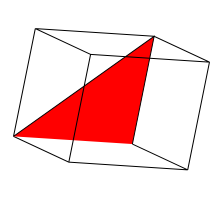
\includegraphics[scale=0.5]{figures/filling.png}
\caption{TODO. Can we find a simple triangulation or just simplification to use the fill() method on strictly convex sets?}

\end{figure}
\end{flushleft}


Convex sets contain the path between two points inside the set. That means, that the direct way from a to be is not crossing the borders of the set. This can be imagined with real borders of a set. A round set, or a rectangle have all points inside together with their path. A star for example, where you have two points at two of the tips is not convex, the direct path, the straight line would cross the border of the star, leave the star, and reenter the star. There is a formula, which gives the points on the path.

\begin{displaymath}
u = \lambda\vec{x} + (1-\lambda)\vec{y}, \lambda \in [0,1], x,y \in V \implies u \in V
\end{displaymath}

The factor lambda lies between 0 and 1. If $\lambda = 0.1$ then is $(1-\lambda) = 0.9$, if $\lambda = 0.2$ then is $(1-\lambda) = 0.8$ and so on. The result is lying on the straight line between $\vec{x}$ and $\vec{y}$. I have taken two vectors $\vec{x}, \vec{y} \in R^2$ and drawn them. The points lie on the line between the two points.

There is an inequality, which convex functions have to satisfy. And you may know it. It is the \emph{triangle inequality}

\begin{displaymath}
\|\lambda\vec{x} + (1-\lambda)\vec{y}\| \leq \lambda\|\vec{x}\| + (1-\lambda)\|\vec{y}\|
\end{displaymath}

or what expresses, that a function is convex.

\begin{displaymath}
f(\lambda\vec{x} + (1-\lambda)\vec{y}) \leq \lambda f(\vec{x}) + (1-\lambda)f(\vec{y})
\end{displaymath}

What is again the \emph{triangle inequality}.

Our image is very precise, because we designed a real coordinate system. What is happening to our new vector? 

\begin{displaymath}
\lambda\boldsymbol{A}\vec{x} + (1-\lambda)\boldsymbol{A}\vec{y} = \boldsymbol{A}(\lambda\vec{x} + (1-\lambda)\vec{y})
\end{displaymath}

By the rule of linearity.


\section{Definition of \mathbb{R}^{2\times3} (WORKING ON)}


\subsection{Defining the $(2\times3)\cdot(3\times1)$ as transitional operation to go from 3-D to 2-D}

The $\mathbb{R}^{2\times3}$ is a K-vectorspace. \\

It has scalar multiplication

\begin{displaymath}
(\lambda, \vec{x}) \mapsto \lambda\vec{x} 
\end{displaymath}

It has addition.

\begin{displaymath}
(\vec{u}, \vec{y}) \mapsto \vec{u} + \vec{x}
\end{displaymath}

You can add 2x3 matrices to 2x3, subtract 2x3 matrices from 2x3 matrices.
The addition of 2x3 matrices stays in the same subspaces.\\

The multiplication of the 2x3 matrices from the left or from the right changes to
the dimension of the resulting matrix.\\

The rule of thumb for matrix multiplication is $(m\times c)\cdot(c\times n)=(m\times n)$.\\

Here we multiply from the left, our 2x3 matrix is the right operand.\\

\begin{tabular}{-l-l-l-l-}
Left Operand & Right Operand & Resultant & Example\\
1x2 & 2x3 & 1x3&\\
2x2 & 2x3 & 2x3&\\
3x2 & 2x3 & 3x3&\\
4x2 & 2x3 & 4x3&\\
\end{tabular}\\

Here we multiply with the right, our matrix is the left operand.\\

\begin{tabular}{-l-l-l-}
Left Operand & Right Operand & Resultant\\
\textbf{2x3} & \textbf{3x1} & \textbf{2x1}& 3-D to 2-D mapping\\
2x3 & 3x2 & 2x2&\\
2x3 & 3x3 & 2x3&\\
2x3 & 3x4 & 2x4& \\
\end{tabular}\\

In my corollary about converting 4 dimensions onto the plane, there is this operation.

\begin{tabular}{-l-l-l-}
Left Operand & Right Operand & Resultant\\
\textbf{2x4} & \textbf{4x1} & \textbf{2x1}& 4-D to 2-D mapping\\
\end{tabular}\\

\newtheorem{PropositionOpt1}{Proposition. The $\mathbb{R}^{2\times3}$ operators have infinite combination possibilities $(m\times c)\cdot(c\times n)=(m\times n)$}
\begin{PropositionOpt1}
TODO
\end{PropositionOpt1}

Well, we are not alone in R2x3 with our coordinate transformation.\\

But. I want to come back to the main definition. \\

\newtheorem{PropositionOpt2}{Proposition. The $2\times3$ matrix operator is optimal for transforming 3-D into 2-D.}
\begin{PropositionOpt2}
With three coordinate axes as column vectors, arranged around the circle, deriving from the 2x3 standard basis with one linearly combined axis vector out of three, and a maximum of three linearly combined basis vectors by arrangement around the circle, the 2x3 matrix is an optimal operator for transforming 3x1 vectors (3-D vectors) into 2x1 vectors (2-D vectors).
\end{PropositionOpt2}

Remark. Got to prove it. Will find a good proof for.
\newtheorem{PropositionOpt4}{Proposition. Definition. Non-Standard Basis.}
\begin{PropositionOpt3}
A non-standard basis is something, which behaves like a basis, but is not a basis after the theorems. For example are the three axis vectors of the 2x3 matrix which transform and map three dimensions onto a 3-D coordinate system on the 2-D plane are a non-standard basis.
\end{PropositionOpt3}

\newtheorem{PropositionOpt4}{Proposition. Definition. 2x3 Non-Standard Basis.}
\begin{PropositionOpt4}
The first two intuitive non-standard basess for the 2x3 is the 90-degree $xy$ and 45 or 225 degree for $z$ combination, which has the values of the 2-D standard basis on two axes and a third one being exactly in the middle of both pointing into positive or negative direction with a value of $\pm\frac{1}\sqrt{2}$ or $\pm2^{-\frac12}$. The third one has an angle of 120 degrees between the axes and is arranged around the circle. The theorem is not finished.
\end{PropositionOpt3}

\newtheorem{PropositionOpt5}{Proposition. The $2\times3$ non-standard basis is the optimal 3-D coordinate system for the 2-D space.}
\begin{PropositionOpt5}
Modeled after a 3-D coordinate system on a piece of paper. Seen as a two dimensional image with two dimensional vectors. The 2x3 coordinate system is arranged as three vectors. One can arrange them around a circle using sine and cosine. The transformation brings a perfect linear mapping along the three vectors. The operation is moving the point from zero to the final point. The movements are decomposed into three horizontal and three vertical moves, where the coordinate is the scalar multiple of the axis vector each move.
\end{PropositionOpt5}

Ok. I have to formulate this out again.

\newtheorem{PropositionOpt6}{Proposition. The linear dependent vector can not be removed from the 2x3 basis.}
\begin{PropositionOpt6}
The 2x3 basis can not be reduced to the 2x1 basis with linear independent vectors, because the linear combination with the third vector is required to mix the coordinates for the image.
\end{PropositionOpt6}

Remark. TODO
Remark. (Lost the words i had in the bus)



\subsection{Orthogonality in the 2x3 matrix}


The 2x3 is mapping the 3-D input from $\begin{pmatrix}1&0&0\\0&1&0\\0&0&1\end{pmatrix}$ onto a 2-D plane. The 2-D plane itself follows the rules of orthogonal basis vectors. The standard basis for the R2 is $\begin{pmatrix}1&0\\0&1\end{pmatrix}$. Onto this basis the output of the 2x3 operators will be mapped.\\

Each of the three input coordinates, which regularly come from an orthogonal 3-D system, contributes a piece of movement to the two dimensions of the target space. One move is left or right, by cosine, and one is up or down by sine. On the plane the move is in a right angle against the other.\\

The 2x3 is combining 3 inputs into 2 outputs with $x\vec{e}_x + y\vec{e}_y + z\vec{e}_z$ by using the 2-D veectors as basis for the linear combinations.\\

The 2 outputs are then interpreted by the R2 standard basis as a linear combination of $\mu\begin{pmatrix}1\\0\end{pmatrix}+\nu\begin{pmatrix}0\\1\end{pmatrix}$.

\subsection{Orthogonal Projection from above}

To keep the orthogonality and orthogonal projection be two different words for two different things i add the paragraph directly here. An orthogonal projection is the shortest path from the point in 3-space to the 2-space plane. This is always the right angle directly onto the plane. This is the orthogonal projection, not to be intermingled with the orthogonal basis vectors being right angled. 

\subsubsection{Gram-Schmidt Orthogonalization}
\label{gram_schmidt_excercise}
We have not tried to orthogonalize the three axis vectors yet. In \cite{Strang1} one can read, how to do it.\\

From $\vec{e}_{n}$ we will calculate $\vec{q}_{n}$, the orthogonalized versions of the three axis vectors.\\

Our first vector is easy and just normalized. Using no r-value gives us the e-vector already normalized, but let us get through the three vectors.\\

\begin{displaymath}
\vec{q}_1 = \vec{e}_{x}/\|\vec{e}_{x}\|
\end{displaymath}

Now for the second vector. We remove the linear parts of the first from the second vector with $(q_{1}^{t}\vec{e}_{y})q_{1}$. (Maybe you recognize ($\vec{q}_{1}|\vec{e}_{y})\vec{q}_{1}$) from the orthogonal projection in Hilbert spaces.) In the second step the new vector is normalized by division by its magnitude

\begin{displaymath}
\begin{align}
\vec{b} &= \vec{e}_y - (\vec{q}_{1}^{T}\vec{e}_{y})\vec{q}_{1}\\
\vec{q}_{2} &= \frac{\vec{b}}{\|\vec{b}\|}
\end{align}
\end{displaymath}

And for the third vector we remove the linear parts of the other two vectors and normalize in the second step.

\begin{displaymath}
\begin{align}
\vec{c} &= \vec{e}_{z} - (\vec{q}_{1}^{T}\vec{e}_{z})\vec{q}_{1} - (\vec{q}_{2}^{T}\vec{e}_{z})\vec{q}_{2}\\
\vec{q}_{3} &= \frac{\vec{c}}{\|\vec{c}\|}
\end{align}
\end{displaymath}

Now we have three new vectors. In a $n\times n$ system, they will be linearly independent and form an orthogonal basis.\\


\textbf{Example. Righthand basis}\\

Consider this matrix:

\begin{displaymath}
    E^{\mathbb{R}^{2\times{3}}}_{y\perp z} = \begin{pmatrix}-2^{-\frac12}&0&1\\-2^{-\frac12}&1&0\end{pmatrix}
\end{displaymath}

This is the coordinate system with z-axis up, x pointing 225 degrees down south west, and y to the right.
On a piece of paper i applied Gram-Schmidt.

\begin{displaymath}
\begin{align}
\vec{e}_{x} &= \begin{pmatrix}-\sqrt{\frac12}\\-\sqrt{\frac12}\end{pmatrix}\\
\vec{e}_{y} &= \begin{pmatrix}1\\0\end{pmatrix}\\
\vec{e}_{z} &= \begin{pmatrix}0\\1\end{pmatrix}
\end{align}
\end{displaymath}

Remember. $-2^{-\frac12}$ is the same as $\cos 225$ and $\sin 225$. The length of this vector is already 1.

\begin{displaymath}
\begin{align}
\vec{e}_{x} &= \begin{pmatrix}-\sqrt{\frac12}\\-\sqrt{\frac12}\end{pmatrix}\\
\vec{q}_{1} &= \frac{\vec{e}_{x}}{\|\vec{e}_{x}\|} = \vec{e}_{x}
\end{align}
\end{displaymath}

Now for the second vector\\

\begin{displaymath}
\begin{align}
\vec{e}_{y} &= \begin{pmatrix}1\\0\end{pmatrix}\\
	\vec{b} &= \begin{pmatrix}1\\0\end{pmatrix} - 
	(\begin{pmatrix}-\sqrt{\frac12}&-\sqrt{\frac12}\end{pmatrix}
	\begin{pmatrix}1\\0\end{pmatrix})
	\begin{pmatrix}-\sqrt{\frac12}\\-\sqrt{\frac12} \end{pmatrix}\\
	&= \begin{pmatrix}\frac12\\-\sqrt{\frac12}\end{pmatrix}\\
	\vec{q}_{2} &= \frac{\vec{b}}{\|\vec{b}\|}
			= \begin{pmatrix}\frac{\frac12}{\frac14 + \frac12}\\\frac{-\sqrt{\frac12}}{\frac34}\end{pmatrix} 
			= \begin{pmatrix}\frac23\\-\frac43 \sqrt{\frac12}\end{pmatrix}\\    
\end{align}
\end{displaymath}

And for the third vector.\\

\begin{displaymath}
\begin{align}
\vec{e}_{y} &= \begin{pmatrix}0\\1\end{pmatrix}\\
\vec{c} &= \vec{e}_{z} - (\vec{q}_{1}^{T}\vec{e}_{z})\vec{q}_{1} - (\vec{q}_{2}^{T}\vec{e}_{z})\vec{q}_{2}\\
			&= \begin{pmatrix}0\\1\end{pmatrix} - \begin{pmatrix}\frac12\\\frac12\end{pmatrix}-(-\frac43\sqrt{\frac12})\begin{pmatrix}\frac46\\-\frac43\sqrt{\frac12}\end{pmatrix}\\
\vec{q}_{3} = \frac{\vec{c}}{\|c\|}
			&= \begin{pmatrix}-\frac{25}{18}\\-\frac{7}{18}\end{pmatrix}
\end{align}
\end{displaymath}

Gram Schmidt gave us these vectors.
\begin{displaymath}
\begin{align}
\vec{q}_{1} &=  \begin{pmatrix}-\sqrt{\frac12}\\-\sqrt{\frac12}\end{pmatrix}\\
\vec{q}_{2} &= \begin{pmatrix}\frac46\\-\sqrt{\frac{8}{9}}\end{pmatrix}\\
\vec{q}_{3} &= \begin{pmatrix}-\frac{25}{18}\\-\frac{7}{18}\end{pmatrix}
\end{align}
\end{displaymath}



\subsubsection{Screenshot of after Gram-Schmidt}

I decided to take the 45 degree perspective projection of a cube. I patched the code and the implement.js\\

\begin{figure}[ht]
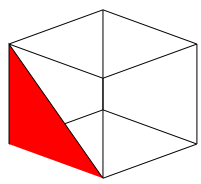
\includegraphics[scale=0.5]{figures/b4ortho.png}
\caption{Before Gram Schmidt. This is the 45 degree lefthand basis.}
\end{figure}

I do not know how big the error of the used source code is. My second screenshot, typing handwritten results in, is not there yet.\\

\begin{figure}[ht]
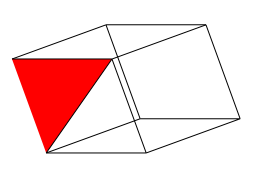
\includegraphics[scale=0.5]{figures/afterortho.png}
\caption{After Gram Schmidt. It seems very fine for this experiment. The angles have changed. But it is very fine when rotated. }
\end{figure}

I do not clean up the code today. This is the little patch, with which i went over my axis vectors. The perspective changes a little, and it is still wonderful. \\


\textbf{Example} JavaScript example code without any error correction. So this is NOT exact. But gives a wonderful insight.

\begin{lstlisting}
function gs_ortho(ex,ey,ez) {
    var norm_ex = norm(ex,2);
    var q1 = [ ex[0]/norm_ex, ex[1]/norm_ex ];
    var tmp = (q1[0] * ey[0] + q1[1] * ey[1]); // q1^t*ey
    var b = [ ey[0] - (tmp*q1[0]),
	      ey[1] - (tmp*q1[1]) ];
    var norm_b = norm(b,2);
    var q2 = [b[0]/norm_b, b[1]/norm_b];
    var tmp1 = (q1[0] * ez[0] + q1[1] * ez[1]);
    var tmp2 = (q2[0] * ez[0] + q2[1] * ez[1]);
    var c = [
	ez[0] - (tmp1*q1[0]) - (tmp2*q2[0]),
	ez[1] - (tmp1*q1[1]) - (tmp2*q2[1])
    ];
    var norm_c = norm(c,2);
    var q3 = [
	c[0]/norm_c, c[1]/norm_c
    ];
    return [q1,q2,q3];
}
\end{lstlisting}



\subsection{Intuitive standard basis for multiplying with 3x1}
\label{intuitive_standard_basis}
First off, the optimal non-standard basis is still arranged around the circle, like at the beginning explained.\\

Remark. When talking of a basis here, we talk with a background of knowing that this is not a linear independent vector space basis, but the only right coordinate system, which is used like a basis, which induces a linear map or a linear combination of three vectors on two dimensions.\\

When deducing from the format of the R2x3 basis, the first suggestions are to use zeros and ones for the basis. The very intuitive first guess using our already defined lefthanded and righthanded systems are these:\\

\begin{displaymath}
    E^{\mathbb{R}^{2\times{3}}}_{lefthand} = \begin{pmatrix}1&0&1\\0&1&1\end{pmatrix} \mbox{ and }
    E^{\mathbb{R}^{2\times{3}}}_{righthand} = \begin{pmatrix}-1&1&0\\-1&0&1\end{pmatrix}
\end{displaymath}

The thing is, the vectors are not normalized in that case (see \ref{why_normalize} for an example, why normalization is sometimes required). We have to do so. If we have two ones, the squared sum is two. The square root out of two is the square root of two. $2^{-\frac12}$ is the normalized length of a vector containing two ones.\\

What else can you see? The standard basis of $\mathbb{R}^{2}$ embedded in the $\mathbb{R}^{2\times3}$ matrix.\\

\begin{displaymath}
    E^{\mathbb{R}^{2\times{3}}}_{x\perp y} = \begin{pmatrix}1&0&2^{-\frac12}\\0&1&2^{-\frac12}\end{pmatrix} \mbox{ and }
    E^{\mathbb{R}^{2\times{3}}}_{y\perp z} = \begin{pmatrix}2^{-\frac12}&0&1\\2^{-\frac12}&1&0\end{pmatrix} \mbox{ and }
    E^{\mathbb{R}^{2\times{3}}}_{x\perp z} = \begin{pmatrix}1&2^{-\frac12}&0\\0&2^{-\frac12}&1\end{pmatrix} 
\end{displaymath}

Can you spot, what i did? I embedded the third axis in some orthogonal 2-D system. Here the axes point into the same positive direction, this is a lefthand system. We look from the back into the z direction.


\begin{displaymath}
    E^{\mathbb{R}^{2\times{3}}}_{x\perp y} = \begin{pmatrix}1&0&-2^{-\frac12}\\0&1&-2^{-\frac12}\end{pmatrix} \mbox{ and }
    E^{\mathbb{R}^{2\times{3}}}_{y\perp z} = \begin{pmatrix}-2^{-\frac12}&0&1\\-2^{-\frac12}&1&0\end{pmatrix} \mbox{ and }
    E^{\mathbb{R}^{2\times{3}}}_{x\perp z} = \begin{pmatrix}1&-2^{-\frac12}&0\\0&-2^{-\frac12}&1\end{pmatrix} 
\end{displaymath}

Here the additional axis shows in the other direction. This is a righthand system. We look from the front against the x direction.
Which is pointing towards us, left down. The y axis is pointing to the right and the z axis to the up.\\

\textbf{With the dot product we test for linear independence}\\

To test the linear independence of two vectors, their dot product must equal zero.\\
That means, the two vectors are perpendicular $\perp$ to each other. They meet in a right angle. As you already know, 
in our 2x3 system it is not possible to give three independent vectors. You can have one to three linear combinations.\\


In our coordinate system, we have to test for $\vec{e}_{x}\cdot\vec{e}_{y}$, $\vec{e}_{x}\cdot\vec{e}_{z}$ and $\vec{e}_{y}\cdot\vec{e}_{z}$.

We test the "embedded" coordinate system with the $\mathbb{R}^{2}$ standard basis and the one linear dependent vector. We 
get another stoking result containing parts of our axis vectors, of course.\\

For the righthand system:\\

\begin{displaymath}
\begin{align}
\vec{e}_{x}\cdot\vec{e}_{y} &= -2^{-\frac12}*1 + -2^{-\frac12}*0 = -2^{-\frac12} = \cos225^{\circ}\\
\vec{e}_{x}\cdot\vec{e}_{z} &= -2^{-\frac12}*0 + -2^{-\frac12}*1 = -2^{-\frac12} = \sin225^{\circ}\\
\vec{e}_{y}\cdot\vec{e}_{z} &= 1*0+0*1 = 0\\
\end{align}
\end{displaymath}

Only the third pair is orthogonal. Two pairs are not. And that in the best case config for orthogonality.\\

For the lefthand system:\\

\begin{displaymath}
\begin{align}
\vec{e}_{x}\cdot\vec{e}_{y} &= 1*0+0*1 = 0\\
\vec{e}_{x}\cdot\vec{e}_{z} &= 1*2^{-\frac12} + 0*2^{-\frac12} = 2^{-\frac12} = \cos45^{\circ}\\
\vec{e}_{y}\cdot\vec{e}_{z} &= 0*2^{-\frac12} + 1*2^{-\frac12} = 2^{-\frac12} = \sin45^{\circ}\\
\end{align}
\end{displaymath}

Only the first pair is orthogonal. The other result in the sin and cosine parts, one for one of the two pairs, due to the mix with the orthogonal pair.\\

\subsection{Deconstructing the 2x3 basis} 

\fbox{The whole section about R2x3 is to be continued very soon}

Remark. This example concerning the book \cite{Strang1} seems to be about R6 and not to match my interpretation.\\

In the Appendix of \cite{Strang1}, there is a basis of a 2x3 matrix printed, together with a few arguments. The professor constructed a 2x3 standard basis by multiplying the 2-D standard basis vectors with the 3-D standard vectors. A 2x3 basis is a set of six matrices being constructed out of five basis vectors according to the books. \\

\begin{displaymath}
\begin{center}
e_{1}^{\mathbb{R}^{2}} = \begin{pmatrix}1\\0\end{pmatrix}
e_{2}^{\mathbb{R}^{2}} = \begin{pmatrix}0\\1\end{pmatrix}\\

e_{1}^{\mathbb{R}^{3}} = \begin{pmatrix}1\\0\\0\end{pmatrix}
e_{2}^{\mathbb{R}^{3}} = \begin{pmatrix}0\\1\\0\end{pmatrix}
e_{2}^{\mathbb{R}^{3}} = \begin{pmatrix}0\\0\\1\end{pmatrix}

\end{center}
\end{displaymath}

Multiplying $e_{i}^{\mathbb{R}^{2}}$ with $(e_{j}^{\mathbb{R}^{3}})^{T}$ yields six independent matrices, which, when added, form the standard basis.

\begin{displaymath}
E^{\mathbb{R}^{2\times{3}}} =
\begin{pmatrix}1&0&0\\0&0&0\end{pmatrix}+
\begin{pmatrix}0&1&0\\0&0&0\end{pmatrix}+
\begin{pmatrix}0&0&1\\0&0&0\end{pmatrix}+
\begin{pmatrix}0&0&0\\1&0&0\end{pmatrix}+
\begin{pmatrix}0&0&0\\0&1&0\end{pmatrix}+
\begin{pmatrix}0&0&0\\0&0&1\end{pmatrix}

\end{displaymath}

Replacing the ones with variables, we get the following.

\begin{displaymath}
\begin{center}
e_{1}^{\mathbb{R}^{2}} = \begin{pmatrix}u\\0\end{pmatrix}
e_{2}^{\mathbb{R}^{2}} = \begin{pmatrix}0\\v\end{pmatrix}\\
e_{1}^{\mathbb{R}^{3}} = \begin{pmatrix}a\\0\\0\end{pmatrix}
e_{2}^{\mathbb{R}^{3}} = \begin{pmatrix}0\\b\\0\end{pmatrix}
e_{2}^{\mathbb{R}^{3}} = \begin{pmatrix}0\\0\\c\end{pmatrix}\\
E^{\mathbb{R}^{2\times{3}}} =
\begin{pmatrix}ua&0&0\\0&0&0\end{pmatrix}+
\begin{pmatrix}0&ub&0\\0&0&0\end{pmatrix}+
\begin{pmatrix}0&0&uc\\0&0&0\end{pmatrix}+
\begin{pmatrix}0&0&0\\va&0&0\end{pmatrix}+
\begin{pmatrix}0&0&0\\0&vb&0\end{pmatrix}+
\begin{pmatrix}0&0&0\\0&0&vc\end{pmatrix}
\end{center}
\end{displaymath}
Here we can subtitute
\begin{displaymath}
ua=r_x\cos\varphi_x,
va=r_x\sin\varphi_x,
ub=r_y\cos\varphi_y,
vb=r_y\sin\varphi_y,
uc=r_z\cos\varphi_z,
vc=r_z\sin\varphi_z,
\end{displaymath}
It should result in
\begin{displaymath}
\begin{center}
\begin{pmatrix}r_x\cos\varphi_x&0&0\\0&0&0\end{pmatrix}+
\begin{pmatrix}0&r_y\cos\varphi_y&0\\0&0&0\end{pmatrix}+
\begin{pmatrix}0&0&r_z\cos\varphi_z\\0&0&0\end{pmatrix}+\\
\begin{pmatrix}0&0&0\\r_x\sin\varphi_x&0&0\end{pmatrix}+
\begin{pmatrix}0&0&0\\0&r_y\sin\varphi_y&0\end{pmatrix}+
\begin{pmatrix}0&0&0\\0&0&r_z\sin\varphi_z\end{pmatrix}\\
   = \begin{pmatrix}
    r_x\cos\varphi_x & r_y\cos\varphi_y & r_z\cos\varphi_z \\
    r_x\sin\varphi_x & r_y\sin\varphi_y & r_z\sin\varphi_z \\
    \end{pmatrix}
\end{center}
\end{displaymath}

That does not solve the problem. It is my first guess from the day, where i spotted the example.\\

\section{Proving more rules of the main formula TODO}

The 'hardest' part is the SVD of the rectangular matrix. I suspect the axis vectors to be the results, but can not prove until i calculate. And i suspect, that every angle changes the singular values, like it changes the eigenvalues of AAt and AtA.\\

The SVD is not that hard. Hard is the handwritten version without numbers with the trigonometric functions, because the terms become very long, and maybe substitution is neccessary to write. I will fix it soon.\\

\subsection{Transpose and TODO}

A 2x3 matrix also has a transpose. Multiplying both result in two different square matrices. $\boldsymbol{A}^T\boldsymbol{A}$ is a 3x3 matrix. And $\boldsymbol{A}\boldsymbol{A}^T$ is a 2 by 2 matrix.\\

\begin{displaymath}
\left(
    \begin{array}{111}
    r_x\cos(\varphi_x) & r_y\cos(\varphi_y) & r_z\cos(\varphi_z) \\
    r_x\sin(\varphi_x) & r_y\sin(\varphi_y) & r_z\sin(\varphi_z) \\
    \end{array}
\right)^T
= \left(
    \begin{array}{11}
    r_x\cos(\varphi_x) & r_x\sin(\varphi_x)\\
    r_y\cos(\varphi_y) & r_y\sin(\varphi_y)\\
    r_z\cos(\varphi_z) & r_z\sin(\varphi_z) \\
    \end{array}
\right)
\end{displaymath}\\

Multiplying out the transposes yield the following forms.\\

$\boldsymbol{A}\boldsymbol{A}^T$, a 2 by 2 matrix.\\

\begin{displaymath}
\boldsymbol{A}\boldsymbol{A}^T = \begin{pmatrix} 
\sum_{i=1}^{3}r_{n}^2\cos^{2}\varphi_{n} & \sum_{i=1}^{3}r_{n}^2\cos\varphi_{n}\sin\varphi_{n}\\
\sum_{i=1}^{3}r_{n}^2\cos\varphi_{n}\sin\varphi_{n} & \sum_{i=1}^{3}r_{n}^2\sin^{2}\varphi_{n}
\end{pmatrix} = \begin{pmatrix}a & b\\b & c
\end{pmatrix}

In the 2x2 matrix $\boldsymbol{A}\boldsymbol{A}^T$ is $a_{ij} = a_{ji}$. 


I will abbreviate $\cos \varphi_{n}$ with $C_{n}$ and
$\sin \varphi_{n}$ with $S_{n}$.\\

$\boldsymbol{A}^T\boldsymbol{A}$ a 3x3 matrix\\

\begin{displaymath}
\boldsymbol{A}^T\boldsymbol{A} = \begin{pmatrix} 
    C_x^2+S_x^2 & C_xC_y+S_xS_y & C_xC_z+S_xS_z\\
    C_yC_x+S_yS_x & C_y^2+S_y^2 & C_yC_z+S_yS_z\\
    C_zC_x+S_zS_x & C_zC_y+S_zS_y & C_z^2+S_z^2
\end{pmatrix}
= \begin{pmatrix}
    r_x^2 & a & b \\
    a & r_y^2 & c \\ 
    b & c & r_z^2 \\
\end{pmatrix}
\end{displaymath}

Also in the 3x3 matrix $\boldsymbol{A}^T\boldsymbol{A}$ is $a_{ij} = a_{ji}$. 

A little bit refined the 3x3 matrix becomes this. Also, to forget about $r_n$ is $r_n = 1$.

\begin{displaymath}
\boldsymbol{A}^T\boldsymbol{A} = \begin{pmatrix}
    1 & \sin(\varphi_x+\varphi_y) & \sin(\varphi_x+\varphi_z) \\
    \sin(\varphi_x+\varphi_y) & 1 & \sin(\varphi_y+\varphi_z) \\ 
    \sin(\varphi_x+\varphi_z) & \sin(\varphi_y+\varphi_z) & 1 \\
\end{pmatrix}
\end{displaymath}


\textbf{Remark} Missing are $|\boldsymbol{A}\boldsymbol{A}^T|$ and $|\boldsymbol{A}^T\boldsymbol{A}|$ and $(\boldsymbol{A}\boldsymbol{A}^T)^{-1}$ and $(\boldsymbol{A}^T\boldsymbol{A})^{-1}$ and various tries to combine them to $P$ = $\boldsymbol{A}(\boldsymbol{A}^T\boldsymbol{A})^{-1}\boldsymbol{A}^T$.\\

The determinant of the
A 2x2 determinant and inverse have the following formulas.

\begin{displaymath}
\begin{align}
\boldsymbol{A} &= \begin{pmatrix}a&b\\c&d\end{pmatrix}\\
|\boldsymbol{A}| &= \det(A) = \begin{vmatrix}a&b\\c&d\end{vmatrix} = ad-bc\\
\boldsymbol{A}^{-1} &= \frac{1}{ad-bc}\begin{pmatrix}d&-b\\-c&a\end{pmatrix}\qquad{, ad-bc \neq 0}
\end{align}
\end{displaymath}


A 3x3 determinant and inverse have the following formulas.

\begin{displaymath}
\end{displaymath}






\subsubsection{Singular Value Decomposition}

TODO\\

This a mxm orthogonal times nxm diagonal times nxn orthogonal. To get the orthogonal we have to take the eigenvectors from the products with the transpose. TODO.\\

\begin{displaymath}
    \boldsymbol{A} = \boldsymbol{U}\boldsymbol{\Sigma}\boldsymbol{V}^{T}
\end{displaymath}

Remark. A rectangular matrix has no eigenvalue equation. But there is a singular value decomposition, which can tell some proper things about the matrix. For that, the eigenvalues are taken from the products with the transpose. And then the decomposition continues.\\

The $A^{T}A$ and $AA^{T}$ are needed for the SVD. First we extract the eigenvalues and eigenvectors of the symmetric square matrices.
$((A^{T}A)-\lambda{I})x=0$ and $((AA^{T})-\lambda{I})x=0$ need to be solved.\\

\subsection{Eigenvalues and -vectors of the 2x2 $AA^{T}$ to reach U}
\label{eig_2x3}

\textbf{Example}
Multiplying the intutitive standard basis from \ref{intuitive_standard_basis} gives

\begin{displaymath}
\boldsymbol{A}\boldsymbol{A}^{T} = \begin{pmatrix}\frac32&\frac12\\\frac12&\frac32\end{pmatrix}
\end{displaymath}

Solving $det(A-\lambda I)=0$ gives us the characteristic polynomial and after foiling and simplification

\begin{displaymath}
\begin{align}
(\frac32-\lambda)^{2}-\frac14\\
=& \lambda^{2}-3\lambda+2\\
=& (\lambda-1)(\lambda-2)
\end{align}
\end{displaymath}

This gives use the poles and the eigenvalues
\begin{displaymath}
\begin{align}
\lambda_{1} &= 1\\
\lambda_{2} &= 2
\end{align}
\end{displaymath}

Subtracting the Eigenvalues from the matrix and solving for the eigenvectors gives me (quick notes from underways on the backside of \cite{Kuehn1})

\begin{displaymath}
\begin{align}
\boldsymbol{A}\boldsymbol{A}^{T}-\lambda_{1}I &= \begin{pmatrix}{\frac12&\frac12\\\frac12&\frac12}\end{pmatrix}\\
\xi_{1} &= \begin{pmatrix}1\\1\end{pmatrix}\\
\boldsymbol{A}\boldsymbol{A}^{T}-\lambda_{2}I &= \begin{pmatrix}{-\frac12&\frac12\\\frac12&-\frac12}\end{pmatrix}\\
\xi_{2} &= \begin{pmatrix}1\\-1\end{pmatrix}\\
\end{align}
\end{displaymath}

This brings me to U of our SVD

\begin{displaymath}
\boldsymbol{U} = \begin{pmatrix}1&1\\1&-1\end{pmatrix}
\end{displaymath}

\subsection{Eigenvalues and -vectors of the 3x3 $A^{T}A$}

\textbf{Possibly wrong}. The determinant could be zero, the polynomial just $(1-\lambda)^{2}$ and the eigenvalues $0,1,1$. The following is from my first notes. The second determinant gave zero, and thinking about gave me the previous results. But now the notes, for the next few days, they are fun in this document.\\

\textbf{Example}\\

After solving for the 2x2 i started solving for the 3x3 with a pen.

\begin{displaymath}
\boldsymbol{A}^{T}\boldsymbol{A} = \begin{pmatrix}1&-2^{-\frac12}&-2^{-\frac12}\\-2^{-\frac12}&1&0\\-2^{-\frac12}&0&1\end{pmatrix}
\end{displaymath}

Underways i subtracted lambda and solved for the determinant using the crossproduct and determinat formula for handwritten determinants of 3x3 matrices.\\

\begin{displaymath}
\boldsymbol{A}^{T}\boldsymbol{A} = \begin{pmatrix}1-\lambda&-2^{-\frac12}&-2^{-\frac12}\\-2^{-\frac12}&1-\lambda&0\\-2^{-\frac12}&0&1-\lambda\end{pmatrix}
\end{displaymath}
By the way. My notes say, the determinant is
\begin{displaymath}
|\boldsymbol{A}^{T}\boldsymbol{A}| = \frac32
\end{displaymath}

Mean, i wanted to fetch the notes, but can not find it. I remember from writing underways, that i only found one pole from
\begin{displaymath}
(1-\lambda)^{2}-(1-\lambda)
\end{displaymath}
which was the result of the determinant minus lambda or the characteristic polynomial. Yes, i only solved the first trivial pole
\begin{displaymath}
\lambda_{2}=1
\end{displaymath}

Solving then for the eigenvector, i got this possible solution for $(\boldsymbol{A}^{T}\boldsymbol{A}-\lambda I)\vec{x}=0$. The first one is 0 because subtracting lamda from the diagonal gave me zero on the whole diagonal.

\begin{displaymath}bb
\boldsymbol{A}^{T}\boldsymbol{A}-\lambda{I} = \begin{pmatrix}0&-2^{-\frac12}&-2^{-\frac12}\\-2^{-\frac12}&0&0\\-2^{-\frac12}&0&0\end{pmatrix}
\end{displaymath}
Solving for the non-zero vector, which results in the zero vector, gives me for $\lambda_{1}$
\begin{displaymath}
\vec{\xi}_{2} = \begin{pmatrix}0\\1\\-1\end{pmatrix}
\end{displaymath}

If this is correct, this is our first eigenvector. If not, i will verify it next time\\

Somewhere here our journey with the bus and subways was over and i have got to come back to the topic soon.\\

On the next morning i looked at the polynomial and got at once the second eigenvalue. It is the zero.
\begin{displaymath}
(1-0)^{2}-(1-0) = 1-1 = 0
\end{displaymath}
So our second eigenvalue, which in order is now the first eigenvalue, is $\lambda_1 = 0$. Installed in our Eigenvector Equation it is just the matrix we started with, because subtracting zero from the diagonal does not change anything.
\begin{displaymath}
(\boldsymbol{A}^{T}\boldsymbol{A}-0I) = \begin{pmatrix}1&-2^{-\frac12}&-2^{-\frac12}\\-2^{-\frac12}&1&0\\-2^{-\frac12}&0&1\end{pmatrix}
\end{displaymath}
Now solve for $(\boldsymbol{A}^{T}\boldsymbol{A}-0I)\vec{x}=0$.
\begin{displaymath}
\end{displaymath}

Oh, and i forgot. A 3x3 polynomial should have three roots. Simplifying $(1-\lambda)^{2}(1-\lambda)$ gives $\lambda^{2}-3\lambda = 0$

\begin{displaymath}
\begin{center}
\lambda^{2}-3\lambda = 0\\
\lambda^{2} = 3\lambda\\
\lambda = 3
\end{center}
\end{displaymath}

So we have all three roots (eigenvalues) together. I have to solve for the remaining two eigenvectors. The 0 value gave a system i still have to solve (underways i started).\\

\begin{displaymath}
\lambda_{1} = 0\qquad\lambda_{2}=1\qquad\lambda_{3}=3
\end{displaymath}

Remark. Nice to get some excercise for this topic.

Remark II. The 3x3 can be mistaken. My last test for the determinant of AtA gave 0, i have to verify this again.

If we have $\boldsymbol{U}$ and $\boldsymbol{V}^{T}$ we can get $\Sigma$ by using $\boldsymbol{A}$
\begin{displaymath}
 \boldsymbol{U}^{T}\boldsymbol{A}\boldsymbol{V} = \boldsymbol{\Sigma}
\end{displaymath}


\subsubsection{The pseudo-inverse $\boldsymbol{A}^{+}$ and least squares}

For a m by n matrix with m < n it is $A^T(AA^{T})^{-1}$\\
For a m by n matrix with m > n it is $(A^{T}A)^{-1}A^T$\\
TODO\\

\section{Computer Error Estimation}

The error $e$ is the absolute value of the exact result $x$ and the computed result $\hat{x}$.

\begin{displaymath}
e = |x - \hat{x}|
\end{displaymath}

In more than one dimension it is the same. The computed result is subtracted from the exact result.

\begin{displaymath}
\vec{e} = \|\vec{x} - \hat{\vec{x}}\|
\end{displaymath}


TODO

Remark. The roundoff error of the floating point and the condition of a matrix is basic knowledge for every computer class.

\section{An alternative graphics algorithm}

\textbf{Remark} This section is new on July 10.

It is obvious, that we want to draw some graphics on our 2-D Canvas. This works on any graphics surface, where you can connect 2-D points with methods, or draw then directly, by changing pixels.

Remark. Missing. The fill algorithm (the stuff is pretty long) and our view frustum (). Plus the remark, we do not try to replace computer graphics. But for small visualizations it is a quick tool, for handwritten code.\\

\subsection{Origin}  

Setting the origin is an easy task. Assuming, the regular origin is at (0,0,0) and (0,0), we just need to add the shift to the coordinate. You can shift the 3-D Origin or the 2-D Origin.  It is just a translation.\\

\begin{lstlisting}
x = Ox + x;
y = Oy + y;
z = Oz + z;
\end{lstlisting}

This has to be applied to every point.

\subsection{Translation}

You simply add the translation vector to each point.\\

Remark. This is the same like shifting the origin, but translation has a meaning, that it is then done, maybe a few times, with animation, to move from a to b.

\begin{lstlisting}
x = Tx + x;
y = Ty + y;
z = Tz + z;
\end{lstlisting}

Remark. A affine combination is written $x = a + Ax$. So to say, the same for the origin.

\subsection{Scaling}

To scale the object you just have to multiply with the constant. 

\begin{lstlisting}
x = Sx * x;
y = Sy * y;
z = Sz * z;
\end{lstlisting}


\subsection{Skewing}

Skewing or shearing is not difficult. I took a skewing matrix and forgot about the empty fields.

\begin{lstlisting}
u = x, v = y, w = z;
x =      u + k_xy*v + k_xz*w;
y = k_yx*u + v      + k_yz*w;
z = k_zx*u + k_zy*v + w;
\end{lstlisting}

\subsection{Local 3x3 basis for change of units and per object rotation}

If you wish to introduce different units for different directions, you have to apply a local basis, if the picture is moving angular. Applying the local 3x3
basis to an object makes sure, it will be rotatable, but without side effects. If you would change the units of r on the projection, then the rotation will give unrealistic results, since suddenly the object stretches to an unexpected size, when entering the zone. \\

The matrix applied locally is a 3x3 matrix $\begin{pmatrix} xBX & yBX & zBX\\ xBY & yBY & zBY\\ xBZ & yBZ & zBZ\end{pmatrix}$.
For example is $\begin{pmatrix} 1 & 0 & 0\\ 0 & 1 & 0\\ 0 & 0 & 1\end{pmatrix}$ is the original and orthonormal (orthogonal and unit length) standard basis for the $\mathbb{R}^{3}$ and the result is the same as if you do not apply any basis to the object, as the assumed default coordinate system in $\mathbb{R}^{3}$ is orthonormal.\\

\begin{lstlisting}
u = x, v = y, w = z;
x = u*xBX + v*yBX + w*zBX;
y = u*xBY + v*yBY + w*zBY;
z = u*xBZ + v*yBZ + w*zBZ;
\end{lstlisting}

This of course transforms the object by the directions and the length of the three three dimensional basis vectors.

\subsubsection{Creating a 3x3 basis with cross products}
\begin{lstlisting}
function cross(a,b) {
    // does not multiply with the ijk components, diy
    return [a[1]*b[2]-a[2]*b[1],-a[0]*b[2]+a[2]*b[0],a[0]*b[1]-a[1]*b[0]];
}
\end{lstlisting}

// if you look and remember \ref{crossproducts} you see the third determinant only giving (1-0)k
\begin{lstlisting}
var u = [1,0,0];
var v = [0,1,0]; 
var w = cross(u,v);
// w = [0,0,1]
\end{lstlisting}
// if you look and remember \ref{crossproducts} you see the third determinant only giving (-1-0)k
\begin{lstlisting}
var u = [-1,0,0];
var v = [0,1,0];
var w = cross(u,v);
// w = [0,0,-1]
\end{lstlisting}

\subsection{Rotation}

Rotating the object can be done in three dimensional space by applying the regular rotation matrices. 

\begin{lstlisting}
// once
    var rotxcos = Math.cos(xAngleRad), rotxsin = Math.sin(xAngleRad);
    var rotycos = Math.cos(yAngleRad), rotysin = Math.sin(yAngleRad);
    var rotzcos = Math.cos(zAngleRad), rotzsin = Math.sin(zAngleRad);
// for each point
    u = x, v = y, w = z;
    y = v * rotxcos - w * rotxsin
    z = v * rotxsin + w * rotxcos
    u = x, v = y, w = z;
    x =  u * rotycos + w * rotysin;
    z = -u * rotysin + w * rotycos;
    u = x, v = y, w = z;
    x = u * rotzcos - v * rotzsin;
    y = u * rotzsin + v * rotzcos;
\end{lstlisting}

\subsection{Frustum and Perspective}

Apply the perspective to the 3x3 set of points before projecting.

\begin{lstlisting}
TODO
\end{lstlisting}


\subsection{Dot product}

The dot product or inner product or scalar product is the sum of the component products and one of the most important basic formulas in space.\\

\begin{lstlisting}
function dot(a,b) {
    var sum = 0;
    for (var i = 0, j = a.length; i < j; i++) sum += a[i]*b[i];
    return sum;
}
\end{lstlisting}

\subsection{Norm}

The euclidean norm is the length of the vector. It´s the square root pulled out of the sum of all components squared.\\

\begin{lstlisting}
function norm(a) {
    var sum = 0;
    for (var i = 0, j = a.length; i < j; i++) sum += a[i]*a[i];
    return Math.sqrt(sum);
}
\end{lstlisting}\\

A p-Norm version, the second argument is the exponent p and p-th root.\\

\begin{lstlisting}
function norm(a,p) {
    var sum = 0;
    if (p===undefined) p = 2;
    if (p===Infinity) {
        var max = 0;
        for (var i = 0, j = a.length; i < j; i++) {
            max = Math.max(Math.abs(a[i]), max);
        }
        return max;
    }
    for (var i = 0, j = a.length; i < j; i++) sum += Math.pow(Math.abs(a[i]),p);
    for (i = 2; i <= p; i++) sum = Math.sqrt(sum);
    return sum;
}
\end{lstlisting}

\subsection {Metric}

The distance function gives us the distance between two points, that is the length of the vector from tip to tip.

\begin{lstlisting}
function d(a,b) {
    var sum = 0;
    for (var i = 0, j = a.length; i < j; i++) sum += Math.pow(a[i]-b[i],2);
    return Math.sqrt(sum);
}
\end{lstlisting}


\subsection{Code Example}

Here is an implementation of these function together with the EcmaScript 6 snippet in modern EcmaScript 5.\\

These functions are not optimized for speed. Each of the -all functions take the whole set of points, so 
the complexity rises to n times iterating over the point sets. To create faster code, you got to inline your
code and do everything in the right order in one loop. Anyways, that is not difficult and intuitive to programmers.\\


\begin{lstlisting}
(function (exports) {

function rad(deg) { 
    return Math.PI/180*deg; 
}

var r_x = 1, r_y = 1, r_z = 1;

var phi_x = rad(210), phi_y = rad(330), phi_z = rad(90);

var xAxisCos = r_x * Math.cos(phi_x),
    yAxisCos = r_y * Math.cos(phi_y),
    zAxisCos = r_z * Math.cos(phi_z),
    xAxisSin = r_x * Math.sin(phi_x),
    yAxisSin = r_y * Math.sin(phi_y),
    zAxisSin = r_z * Math.sin(phi_z);

function transform2d(vec3) {
    return [
    vec3[0]*xAxisCos + vec3[1]*yAxisCos + vec3[2]*zAxisCos,
    vec3[0]*xAxisSin + vec3[1]*yAxisSin + vec3[2]*zAxisSin
    ];
}

function transform2dAll(avec3) {
    return avec3.map(transform2d);
}

function settrans(op) {
    if (op.phi_n) {
    phi_x = op.phi_n[0];
    phi_y = op.phi_n[1];
    phi_z = op.phi_n[2];
    }
    if (op.r_n) {
    r_x = op.r_n[0];
    r_y = op.r_n}[1];
    r_z = op.r_n[2];
    }
    xAxisCos = r_x * Math.cos(phi_x);
    yAxisCos = r_y * Math.cos(phi_y);
    zAxisCos = r_z * Math.cos(phi_z);
    xAxisSin = r_x * Math.sin(phi_x);
    yAxisSin = r_y * Math.sin(phi_y);
    zAxisSin = r_z * Math.sin(phi_z);
}

function gettrans() { 
    return { 
    phi_n: [phi_x, phi_y, phi_z], 
    r_n: [r_x, r_y, r_z] 
    }; 
}

function draw2dAll(ctx, points2, scale) {
    ctx.save();
    scale = scale || 1;
    var x = scale * points2[0][0], y = scale * points2[0][1];
    ctx.moveTo(x,-y);
    ctx.beginPath();
    for (var i = 0, j = points2.length; i < j; i++) {
    x = scale * points2[i][0], y = scale * points2[i][1];
    ctx.lineTo(x,-y);
    ctx.moveTo(x,-y);
    }
    ctx.closePath();
    ctx.stroke();
    ctx.restore();
}

function rotate3dAll(xAngleRad,yAngleRad,zAngleRad, points3) {
    var rotxcos = Math.cos(xAngleRad), rotxsin = Math.sin(xAngleRad);
    var rotycos = Math.cos(yAngleRad), rotysin = Math.sin(yAngleRad);
    var rotzcos = Math.cos(zAngleRad), rotzsin = Math.sin(zAngleRad);
    var p, x, y, z, u, v, w;
    for (var i = 0, j = points3.length; i < j; i++) {
        p = points3[i], x = p[0], y = p[1], z = p[2];
        u = x, v = y, w = z;
        y = v * rotxcos - w * rotxsin
        z = v * rotxsin + w * rotxcos
        u = x, v = y, w = z;
        x = u * rotycos + w * rotysin;
        z = -u * rotysin + w * rotycos;
        u = x, v = y, w = z;
        x = u * rotzcos - v * rotzsin;
        y = u * rotzsin + v * rotzcos;
        p[0]=x;
        p[1]=y;
        p[2]=z;
    }
}
    
function rotate2dAll(zAngle, points2) {
    var rotzcos = Math.cos(zAngleRad), rotzsin = Math.sin(zAngleRad);
    var p, x, y, u, v;
    for (var i = 0, j = points2.length; i < j; i++) {
        p = points2[i], x = p[0], y = p[1];
        u = x, v = y;
        x = u * rotzcos - v * rotzsin;
        y = u * rotzsin + v * rotzcos;
        p[0]=x;
        p[1]=y;
    }
}

function translate3dAll(transvec, points3) {
    var p, x, y, z;
    var Tx = transvec[0],
    Ty = transvec[1],
    Tz = transvec[2];
    for (var i = 0, j = points3.length; i < j; i++) {
        p = points3[i];
        p[0]+=Tx;
        p[1]+=Ty;
        p[2]+=Tz;
    }
}

function translate2dAll(transvec, points2) {
    var p;
    var Tx = transvec[0],
    Ty = transvec[1];
    for (var i = 0, j = points2.length; i < j; i++) {
        p = points2[i];
        p[0]+=Tx;
        p[1]+=Ty;
    }
}

function scale3dAll(scaleX, scaleY, scaleZ, points3) {
    var p;
    for (var i = 0, j = points3.length; i < j; i++) {
        p = points3[i];
        p[0]*=scaleX;
        p[1]*=scaleY;
        p[2]*=scaleZ;
    }
}

function scale2dAll(scaleX, scaleY, points2) {
    var p;
    for (var i = 0, j = points2.length; i < j; i++) {
        p = points2[i];
        p[0]*=scaleX;
        p[1]*=scaleY;
    }
}

function compareAll(points3, points2, callback) {
    var results = [];
    for (var i = 0, j = points3.length; i < j; i++) {       
        results.push(callback(points3[i],points2[i]));
    }
    return results;
}

exports.gettrans = gettrans;
exports.settrans = settrans;
exports.transform2d = transform2d;
exports.transform2dAll = transform2dAll;
exports.rotate3dAll = rotate3dAll;
exports.rotate2dAll = rotate2dAll;
exports.scale3dAll = scale3dAll;
exports.scale2dAll = scale2dAll;
exports.translate3dAll = translate3dAll;
exports.translate2dAll = translate2dAll;
exports.compareAll = compareAll;
exports.rad = rad;
exports.draw2dAll = draw2dAll;

}(typeof exports != "undefined" ? exports : this));

\end{lstlisting}

Last but not least here is a code snippet doing all the things together.

\begin{lstlisting}

var n = points3.length;
var i = 0;
while (i < n) {
    var x,y,z, u,v,w;

    // local operations
    translate;
    rotate;
    scale;

    // world operations
    translate;
    rotate;
    scale;

    i++;

}

\end{lstlisting}

\section{How i was wrong the first time. Turning $xy$-around and adding $z$ in.}

Remark. This was the transformation i found before i invented the axes. This brought me to the invention.\\

Before i figured out, how to create three axes, i did it wrong. I wanted to turn three axes around, but did only rotate the $xy$-plane. With the well known formula for rotating around the z-axis in the $\mathbb{R}^{2}$. I tried to combine this for the other axes, but failed. But i had an idea, as the $xy$-axes were pointing downwards. I was writing it on the computer, the hardware $y$-axis was free after rotation. I added the z-coordinate to the y coordinate, believing it would shift the point upwards vertically. I found an interpretation of the righthanded coordinate system.\\

\begin{enumerate}
 \item{Rotate the $xy$-plane by for example 225 degrees or $\frac{\pi}{180}\times225=\frac{15\pi}{12}=\frac{5}{4}\pi = 1.25\pi$ radians.}
 \item{Now the x-axis and the y-axis point downwards. This means, the real y-axis on the real 2-D coordinate system is now 'free'.}
 \item{So add the z-coordinate in by just adding it to y.}
}\\
\end{enumerate}

I will show it again now step by step.\\
The angle to turn each point around.
\begin{displaymath}
\angle{\alpha} = 1.25\pi\\
\end{displaymath}
The rotation matrix for two dimensions, turns the plane around the z-axis. The z-axis points invisible and orthogonally out of the screen to the viewer.
\begin{displaymath}
\boldsymbol{R} = \begin{pmatrix}\cos \angle{\alpha}& -\sin \angle{\alpha} \\ \sin \angle{\alpha} & \cos \angle{\alpha} \end{pmatrix}\\
\end{displaymath}
v is the input vector, and w is the output vector.
\begin{displaymath}
v = (x,y,z)^T, w = (v_1, v_2)^T = (x,y)^T\\
\end{displaymath}
Now we rotate each point containing only the x,y coordinate of the triple v.
\begin{displaymath}
\boldsymbol{R}\left(\begin{array}{1}x\\y\end{array}\right) = \left(\begin{array}{1}x\\y\end{array}\right) = \vec{y}'\\
\end{displaymath}
The x,y image is pointing downwards. I add each point it`s z coordinate now to y. That moves the point upwards by the amount of z.
\begin{displaymath}
\left(\begin{array}{1}x\\y+z\end{array}\right) = \vec{y}''
\end{displaymath}
After this i discovered adding three proportional parts. One for each coordinate. And decided quickly, to use cos and sin and the circle, to create axes by angles.\\

\textbf{Example}\\
This is the EcmaScript 5 code example for rotating xy and addign z in.
\begin{example}
\begin{lstlisting}
function transform(points3) {

    var angle = 1.25*Math.PI;  // 225 deg
    var cos = Math.cos(angle), // prevent to
        sin = Math.sin(angle); // repeat calls to
    var points2 = [];          // new points
    var p;                     // current point
    var x,y,u,w,z;             // coordinates
    
    for (var i = 0, j = points3.length; i < j; i++) {

        p = points3[i];
        u = p[0], 
        v = p[1], 
        z = p[2];

        // rotate x and y 
        x = cos*u -sin*v; 
        y = sin*u +cos*v; 
    
        // add z vertically
        y += z; 
        // could do it on one line with the previous y

        // add new point to list
        points2.push([x,y]);
    }

    return points2;
}
\end{lstlisting}
\end{example}


\section{Declaration of authorship}

German.\\

Ich habe dieses Koordinatensystem selbst entwickelt. Es ist keine Formel aus einem Buch oder einer Lehrveranstaltung.
Ob es irgendwo eine identische Formel oder eine vergleichbare Definition gibt, ist mir nicht bekannt.
Ich habe den Inhalt des Dokuments aus eigenem Ermessen zusammengestellt. Ich habe mir Gedanken zum Thema gemacht und
ausserdem Rechnungen mit Stift und Papier angefertigt. Ausserdem habe ich in Lehrb\"uchern und Veranstaltungen gebl\"attert,
um das Koordinatensystem und die definierten Variabeln und Operationen m\"oglichst gut in die reelle Mathematik einzuordnen.
Mir m\"ogen Fehler unterlaufen sein, und auch Details entgangen sein. F\"ur beides m\"ochte ich mich entschuldigen.\\

English.\\

I habe developed this coordinate system by myself. It is no formula from a book or a class lecture. 
Wether a identical formula or a comparable definition exists, is not known to me.
Ich have collected the content of this document on my own behave. I have made up my mind about the topic
and also created calculations with pen and paper. Also i browsed literature and lectures to insert the
coordinate system and the defined variables and operations likely good into the real mathematics.
Mistakes may have been made by me, and Details may be not have been recognized. For both i would like 
to excuse myself.\\

First version.\\

With this here i promise, i invented the thing alone, and did copy no proof nowhere and used only
the books and the lecture scripts for reference i acknowledge in the bibliography.\\

\section{License}

First.\\

This code is free of charge, free for anyone to use. You are welcome to accredit Edward Gerhold for his work.
But it is not neccessary to do so. I can say it with a rhyme. I did it, too. And explained it to you. However.
You may use it. You may have it. But by the declaration of ownership, i have really developed this all myself.
And i keep it for the people.\\

German. \\

Der produzierte Source Code, um das Koordinatensystem und einige Abbildungen zu zeigen, ist frei f\"ur alle,
wie auch das Koordinatensystem selbst und die dazugeh\"origen Definitionen, die ich selbst angefertigt habe.
Es ist erlaubt, mir daf\"ur Anerkennung zu gew\"ahren, es ist aber nicht zwingend n\"otig, mich daf\"ur im
eigenen Projekt zu nennen. Allerdings mag auch ich keine Menschen, die diese Arbeit f\"ur ihre eigene ausgeben.\\

English.\\

The produced source code, to show the coordinate system and a few maps, is free for all, like the coordinate
sytem itself and the related definitions, i created myself. It is allowed to give me respect for, but it is 
not absolutly neccessary, to put my name into your own projects. Of course i don´t like people, who pretend 
this is already their work.\\

\section{Third-Party Software}

\begin{enumerate}
\item The document has been written for and compiled with pdf\LaTeX.  The tex source is compiled by hitting Strg-B
in SublimeText3 to start a buildscript i have written for.

\item The document source code is part of the zip from the github repository https://github.com/edwardgerhold/paper-pen-3D
The repository name may have changed to /pen-and-paper-3-D or to /2x3-D, if it is no longer reachable under paper-pen-3D.
Until then, it is not sure, that i will change the name, it is in /paper-pen-3D. 

\item For the figures i used the free and platform-independent mathematical software GeoGebra (http://geogebra.org). GeoGebra has much more to give, than the little figures i have drawn with. Incorrect labels on the pictures are due to the novice experience with GeoGebra.

\item The text has been written with a unregistered version of SublimeText, which is one of the great text editors 
available, if you do not directly use a full-featured integrated development environment.

\item The demo implementations use JavaScript and HTML5 and should run in almost all browsers on all platforms having the 
2-D Canvas  available. No WebGL required to show the 3-D transformation. Possibly you see, why the coordinate system
is less known. In my opinion, because computer graphics went a slightly different way, the coordinate system has not
been noticed anymore.
\end{enumerate}


\begin{thebibliography}

\bibitem{Corral1} \textit{Michael Corral, Schoolcraft College},
        Vector Calculus, GNU Free Documentation License, http://mecmath.net\\
    \bibitem{Corral2} \textit{Michael Corral, Schoolcraft College},
        Trigonometry, GNU Free Documentation License, http://mecmath.net 
    \bibitem{Strang1} \textit{Gilbert Strang, MIT},
            Linear Algebra and it´s Applications. Fourth Edition.        
    \bibitem{Strang2} \textit{Gilbert Strang, MIT},
            Calculus. MIT OpenCourseWare Supplemental Resources. http://ocw.mit.edu    
    \bibitem{Toplogy} \textit{John Rogues, Lecture Notes on Topology, following J.R.Munkres Textbook, for MAT3500/4500},
            Lecture Script, Topology (english), http://
    \bibitem{Vershynin1} \textit{Roman Vershynin. Lectures in Functional Analysis. Department of Mathematics, University of Michigan},
            Lecture Script, http://,        
    \bibitem{Ferus1} \textit{Dirk Ferus, TU-Berlin, em.},
            Lecture Script, Lineare Algebra 1+2, 2000, http://page.math.tu-berlin/~ferus/skripten.html
    \bibitem{Kuehn1} \textit{Franziska K\"uhn, Technische Universit\"at Dresden},
            Lecture Script, Lineare Algebra und analytische Geometrie I+II, http://fkuehn.de/download/LAAG.pdf
    \bibitem{Wittbold} \textit{Petra Wittbold, TU-berlin},  
            Lecture Script, Funktionalanalysis I,  http://www3.math.tu-berlin.de/Vorlesungen/SS09/FA1/Doc/Funkana1-SS06-08.06.09.pd
    \bibitem{Corral3} \textit{Michael Corral, Schoolcraft College},
            Latex Mini Tutorial, http://mecmath.net                    
    \bibitem{Jürgens,Feuerstack} \textit{Manuela J\"urgens, Thomas Feuerstack, Fernuniversit\"at Hagen},
            LaTeX, eine Einf\"uhrung und ein bisschen mehr..., a026\_latex\_einf.pdf            
    \bibitem{Rudl} \textit{Dr.Jan Rudl, Technische Universit\"at Dresden, Fachbereich Mathematik},
            Einf\"uhrung in LaTeX, LaTeX-Kurs.pdf            
\end{thebibliography}


\makeindex
\printindex

\end{document}

                                                                                                                                                                                